\documentclass[twoside]{book}

% Packages required by doxygen
\usepackage{fixltx2e}
\usepackage{calc}
\usepackage{doxygen}
\usepackage[export]{adjustbox} % also loads graphicx
\usepackage{graphicx}
\usepackage[utf8]{inputenc}
\usepackage{makeidx}
\usepackage{multicol}
\usepackage{multirow}
\PassOptionsToPackage{warn}{textcomp}
\usepackage{textcomp}
\usepackage[nointegrals]{wasysym}
\usepackage[table]{xcolor}

% Font selection
\usepackage[T1]{fontenc}
\usepackage[scaled=.90]{helvet}
\usepackage{courier}
\usepackage{amssymb}
\usepackage{sectsty}
\renewcommand{\familydefault}{\sfdefault}
\allsectionsfont{%
  \fontseries{bc}\selectfont%
  \color{darkgray}%
}
\renewcommand{\DoxyLabelFont}{%
  \fontseries{bc}\selectfont%
  \color{darkgray}%
}
\newcommand{\+}{\discretionary{\mbox{\scriptsize$\hookleftarrow$}}{}{}}

% Page & text layout
\usepackage{geometry}
\geometry{%
  a4paper,%
  top=2.5cm,%
  bottom=2.5cm,%
  left=2.5cm,%
  right=2.5cm%
}
\tolerance=750
\hfuzz=15pt
\hbadness=750
\setlength{\emergencystretch}{15pt}
\setlength{\parindent}{0cm}
\setlength{\parskip}{3ex plus 2ex minus 2ex}
\makeatletter
\renewcommand{\paragraph}{%
  \@startsection{paragraph}{4}{0ex}{-1.0ex}{1.0ex}{%
    \normalfont\normalsize\bfseries\SS@parafont%
  }%
}
\renewcommand{\subparagraph}{%
  \@startsection{subparagraph}{5}{0ex}{-1.0ex}{1.0ex}{%
    \normalfont\normalsize\bfseries\SS@subparafont%
  }%
}
\makeatother

% Headers & footers
\usepackage{fancyhdr}
\pagestyle{fancyplain}
\fancyhead[LE]{\fancyplain{}{\bfseries\thepage}}
\fancyhead[CE]{\fancyplain{}{}}
\fancyhead[RE]{\fancyplain{}{\bfseries\leftmark}}
\fancyhead[LO]{\fancyplain{}{\bfseries\rightmark}}
\fancyhead[CO]{\fancyplain{}{}}
\fancyhead[RO]{\fancyplain{}{\bfseries\thepage}}
\fancyfoot[LE]{\fancyplain{}{}}
\fancyfoot[CE]{\fancyplain{}{}}
\fancyfoot[RE]{\fancyplain{}{\bfseries\scriptsize Generated by Doxygen }}
\fancyfoot[LO]{\fancyplain{}{\bfseries\scriptsize Generated by Doxygen }}
\fancyfoot[CO]{\fancyplain{}{}}
\fancyfoot[RO]{\fancyplain{}{}}
\renewcommand{\footrulewidth}{0.4pt}
\renewcommand{\chaptermark}[1]{%
  \markboth{#1}{}%
}
\renewcommand{\sectionmark}[1]{%
  \markright{\thesection\ #1}%
}

% Indices & bibliography
\usepackage{natbib}
\usepackage[titles]{tocloft}
\setcounter{tocdepth}{3}
\setcounter{secnumdepth}{5}
\makeindex

% Hyperlinks (required, but should be loaded last)
\usepackage{ifpdf}
\ifpdf
  \usepackage[pdftex,pagebackref=true]{hyperref}
\else
  \usepackage[ps2pdf,pagebackref=true]{hyperref}
\fi
\hypersetup{%
  colorlinks=true,%
  linkcolor=blue,%
  citecolor=blue,%
  unicode%
}

% Custom commands
\newcommand{\clearemptydoublepage}{%
  \newpage{\pagestyle{empty}\cleardoublepage}%
}

\usepackage{caption}
\captionsetup{labelsep=space,justification=centering,font={bf},singlelinecheck=off,skip=4pt,position=top}

%===== C O N T E N T S =====

\begin{document}

% Titlepage & ToC
\hypersetup{pageanchor=false,
             bookmarksnumbered=true,
             pdfencoding=unicode
            }
\pagenumbering{roman}
\begin{titlepage}
\vspace*{7cm}
\begin{center}%
{\Large Traffic Sign Recognition using a Turtlebot }\\
\vspace*{1cm}
{\large Generated by Doxygen 1.8.11}\\
\end{center}
\end{titlepage}
\clearemptydoublepage
\tableofcontents
\clearemptydoublepage
\pagenumbering{arabic}
\hypersetup{pageanchor=true}

%--- Begin generated contents ---
\chapter{Class Index}
\section{Class List}
Here are the classes, structs, unions and interfaces with brief descriptions\+:\begin{DoxyCompactList}
\item\contentsline{section}{\hyperlink{classclassifier}{classifier} \\*Definition of the classifier class. It contains all the functions and variables depicted in the }{\pageref{classclassifier}}{}
\item\contentsline{section}{\hyperlink{classrobot}{robot} }{\pageref{classrobot}}{}
\item\contentsline{section}{\hyperlink{classtestclass}{testclass} \\*Definition of the testclass class. It contains mock callbacks to test publishers and subscribers }{\pageref{classtestclass}}{}
\end{DoxyCompactList}

\chapter{File Index}
\section{File List}
Here is a list of all documented files with brief descriptions\+:\begin{DoxyCompactList}
\item\contentsline{section}{/home/michi/catkin\+\_\+ws/src/traffic\+\_\+sign\+\_\+recognition/include/\hyperlink{classifier_8hpp}{classifier.\+hpp} \\*Header file with definitions for class classifier }{\pageref{classifier_8hpp}}{}
\item\contentsline{section}{/home/michi/catkin\+\_\+ws/src/traffic\+\_\+sign\+\_\+recognition/include/\hyperlink{robot_8hpp}{robot.\+hpp} \\*Header file with definitions for class robot }{\pageref{robot_8hpp}}{}
\item\contentsline{section}{/home/michi/catkin\+\_\+ws/src/traffic\+\_\+sign\+\_\+recognition/src/\hyperlink{classifier_8cpp}{classifier.\+cpp} \\*Implementation of the methods of class classifier }{\pageref{classifier_8cpp}}{}
\item\contentsline{section}{/home/michi/catkin\+\_\+ws/src/traffic\+\_\+sign\+\_\+recognition/src/\hyperlink{navig__node_8cpp}{navig\+\_\+node.\+cpp} \\*Navigation node where all the main functions of the robot behavious happen }{\pageref{navig__node_8cpp}}{}
\item\contentsline{section}{/home/michi/catkin\+\_\+ws/src/traffic\+\_\+sign\+\_\+recognition/src/\hyperlink{robot_8cpp}{robot.\+cpp} \\*Implementation of the methods of class robot }{\pageref{robot_8cpp}}{}
\item\contentsline{section}{/home/michi/catkin\+\_\+ws/src/traffic\+\_\+sign\+\_\+recognition/src/\hyperlink{vision__node_8cpp}{vision\+\_\+node.\+cpp} \\*Vision node where all the main functions of the detection and recognition happen }{\pageref{vision__node_8cpp}}{}
\item\contentsline{section}{/home/michi/catkin\+\_\+ws/src/traffic\+\_\+sign\+\_\+recognition/test/\hyperlink{test__robot_8cpp}{test\+\_\+robot.\+cpp} \\*Unit test code for class robot }{\pageref{test__robot_8cpp}}{}
\item\contentsline{section}{/home/michi/catkin\+\_\+ws/src/traffic\+\_\+sign\+\_\+recognition/test/\hyperlink{test__ros_8cpp}{test\+\_\+ros.\+cpp} \\*Unit tests for publishers and subscribers }{\pageref{test__ros_8cpp}}{}
\item\contentsline{section}{/home/michi/catkin\+\_\+ws/src/traffic\+\_\+sign\+\_\+recognition/test/\hyperlink{test__vision_8cpp}{test\+\_\+vision.\+cpp} \\*Unit test code for classifier class }{\pageref{test__vision_8cpp}}{}
\item\contentsline{section}{/home/michi/catkin\+\_\+ws/src/traffic\+\_\+sign\+\_\+recognition/test/\hyperlink{testclass_8cpp}{testclass.\+cpp} \\*Implementation of the methods of class testclass }{\pageref{testclass_8cpp}}{}
\item\contentsline{section}{/home/michi/catkin\+\_\+ws/src/traffic\+\_\+sign\+\_\+recognition/test/\hyperlink{testclass_8hpp}{testclass.\+hpp} \\*Definition for class testclass }{\pageref{testclass_8hpp}}{}
\end{DoxyCompactList}

\chapter{Class Documentation}
\hypertarget{classclassifier}{}\section{classifier Class Reference}
\label{classclassifier}\index{classifier@{classifier}}


Definition of the classifier class. It contains all the functions and variables depicted in the.  




{\ttfamily \#include $<$classifier.\+hpp$>$}

\subsection*{Public Member Functions}
\begin{DoxyCompactItemize}
\item 
void \hyperlink{classclassifier_a08655fcec6411365a3838ac7c9cd2b19}{image\+Callback} (const sensor\+\_\+msgs\+::\+Image\+Const\+Ptr \&msg)
\begin{DoxyCompactList}\small\item\em The label of the detections, outputed by the S\+VM. \end{DoxyCompactList}\item 
cv\+::\+Mat \hyperlink{classclassifier_a8a7a42fa1bb806e639d23493d5c222d8}{de\+Noise} (cv\+::\+Mat input\+Image)
\begin{DoxyCompactList}\small\item\em Apply gaussian filter to the input image to denoise it. \end{DoxyCompactList}\item 
std\+::vector$<$ cv\+::\+Mat $>$ \hyperlink{classclassifier_a5b5bd9ecfd7fd622b742ee31fafd2f93}{M\+S\+E\+R\+\_\+\+Features} (cv\+::\+Mat img, double \&area)
\begin{DoxyCompactList}\small\item\em Find M\+S\+ER features in the image. First normalize image and binarize, then look for regions and finally, resize each regions image. \end{DoxyCompactList}\item 
cv\+::\+Mat \hyperlink{classclassifier_a162fa849e75034ee7e86b1081de8f3c3}{H\+O\+G\+\_\+\+Features} (cv\+::\+H\+O\+G\+Descriptor hog, std\+::vector$<$ cv\+::\+Mat $>$ imgs)
\begin{DoxyCompactList}\small\item\em Compute the H\+OG features in every image of a vector. \end{DoxyCompactList}\item 
int \hyperlink{classclassifier_af243db8f8ebd929c4cbe6ce9581b06c5}{train\+Stage} (cv\+::\+H\+O\+G\+Descriptor \&hog, cv\+::\+Ptr$<$ cv\+::ml\+::\+S\+VM $>$ \&svm, std\+::vector$<$ cv\+::\+Mat $>$ \&train\+Imgs, std\+::vector$<$ int $>$ \&train\+Labels)
\begin{DoxyCompactList}\small\item\em Function that runs load\+Train\+Imgs(), \hyperlink{classclassifier_a162fa849e75034ee7e86b1081de8f3c3}{H\+O\+G\+\_\+\+Features()} and S\+VM Training, sequentially. \end{DoxyCompactList}\item 
float \hyperlink{classclassifier_ac32914e9de8dc54ed6f803987bf24d25}{S\+V\+M\+Testing} (cv\+::\+Ptr$<$ cv\+::ml\+::\+S\+VM $>$ \&svm, cv\+::\+Mat test\+H\+OG)
\begin{DoxyCompactList}\small\item\em Feed S\+VM with the H\+OG Matrix of the current image and outputs its label. \end{DoxyCompactList}\item 
int \hyperlink{classclassifier_a6cc30b3645926233cbf880c8fa100536}{visualization} ()
\begin{DoxyCompactList}\small\item\em Opens a vindow with the robot\textquotesingle{}s view of the workspace. It outputs bouding box around detected signs and the name of the sign. \end{DoxyCompactList}\end{DoxyCompactItemize}
\subsection*{Public Attributes}
\begin{DoxyCompactItemize}
\item 
cv\+::\+Mat {\bfseries imagen}\hypertarget{classclassifier_a26cdea6917e91262aed520a607eff875}{}\label{classclassifier_a26cdea6917e91262aed520a607eff875}

\item 
std\+::vector$<$ cv\+::\+Rect $>$ \hyperlink{classclassifier_af8f673465c7e37684c3a28a90b8bdc00}{boxes}\hypertarget{classclassifier_af8f673465c7e37684c3a28a90b8bdc00}{}\label{classclassifier_af8f673465c7e37684c3a28a90b8bdc00}

\begin{DoxyCompactList}\small\item\em Open\+CV Image from the camera given by the subscriber. \end{DoxyCompactList}\item 
float \hyperlink{classclassifier_ac13295d3b350ef6c8219004666aeff18}{traffic\+\_\+sign}\hypertarget{classclassifier_ac13295d3b350ef6c8219004666aeff18}{}\label{classclassifier_ac13295d3b350ef6c8219004666aeff18}

\begin{DoxyCompactList}\small\item\em Bounding boxes in the current frame. \end{DoxyCompactList}\end{DoxyCompactItemize}


\subsection{Detailed Description}
Definition of the classifier class. It contains all the functions and variables depicted in the. 

U\+ML Class diagram. It trains a S\+VM, reads images from topic, detects M\+S\+ER and H\+OG features and classifies traffic sign images. 

\subsection{Member Function Documentation}
\index{classifier@{classifier}!de\+Noise@{de\+Noise}}
\index{de\+Noise@{de\+Noise}!classifier@{classifier}}
\subsubsection[{\texorpdfstring{de\+Noise(cv\+::\+Mat input\+Image)}{deNoise(cv::Mat inputImage)}}]{\setlength{\rightskip}{0pt plus 5cm}cv\+::\+Mat classifier\+::de\+Noise (
\begin{DoxyParamCaption}
\item[{cv\+::\+Mat}]{input\+Image}
\end{DoxyParamCaption}
)}\hypertarget{classclassifier_a8a7a42fa1bb806e639d23493d5c222d8}{}\label{classclassifier_a8a7a42fa1bb806e639d23493d5c222d8}


Apply gaussian filter to the input image to denoise it. 


\begin{DoxyParams}{Parameters}
{\em input\+Image} & is the current image to be filtered \\
\hline
\end{DoxyParams}
\begin{DoxyReturn}{Returns}
Blurred and denoised image 
\end{DoxyReturn}
\index{classifier@{classifier}!H\+O\+G\+\_\+\+Features@{H\+O\+G\+\_\+\+Features}}
\index{H\+O\+G\+\_\+\+Features@{H\+O\+G\+\_\+\+Features}!classifier@{classifier}}
\subsubsection[{\texorpdfstring{H\+O\+G\+\_\+\+Features(cv\+::\+H\+O\+G\+Descriptor hog, std\+::vector$<$ cv\+::\+Mat $>$ imgs)}{HOG_Features(cv::HOGDescriptor hog, std::vector< cv::Mat > imgs)}}]{\setlength{\rightskip}{0pt plus 5cm}cv\+::\+Mat classifier\+::\+H\+O\+G\+\_\+\+Features (
\begin{DoxyParamCaption}
\item[{cv\+::\+H\+O\+G\+Descriptor}]{hog, }
\item[{std\+::vector$<$ cv\+::\+Mat $>$}]{imgs}
\end{DoxyParamCaption}
)}\hypertarget{classclassifier_a162fa849e75034ee7e86b1081de8f3c3}{}\label{classclassifier_a162fa849e75034ee7e86b1081de8f3c3}


Compute the H\+OG features in every image of a vector. 


\begin{DoxyParams}{Parameters}
{\em hog} & is the H\+OG Descriptor object with all the parameters set up \\
\hline
{\em imgs} & is the vector of images to get the\+H\+OG from \\
\hline
\end{DoxyParams}
\begin{DoxyReturn}{Returns}
Matrix with the H\+OG Descriptor for all the images. 
\end{DoxyReturn}
\index{classifier@{classifier}!image\+Callback@{image\+Callback}}
\index{image\+Callback@{image\+Callback}!classifier@{classifier}}
\subsubsection[{\texorpdfstring{image\+Callback(const sensor\+\_\+msgs\+::\+Image\+Const\+Ptr \&msg)}{imageCallback(const sensor_msgs::ImageConstPtr &msg)}}]{\setlength{\rightskip}{0pt plus 5cm}void classifier\+::image\+Callback (
\begin{DoxyParamCaption}
\item[{const sensor\+\_\+msgs\+::\+Image\+Const\+Ptr \&}]{msg}
\end{DoxyParamCaption}
)}\hypertarget{classclassifier_a08655fcec6411365a3838ac7c9cd2b19}{}\label{classclassifier_a08655fcec6411365a3838ac7c9cd2b19}


The label of the detections, outputed by the S\+VM. 

Callback used in the subscriber for the camera topic. Gets the R\+OS Img msg and transforms it to an Open\+CV img. 
\begin{DoxyParams}{Parameters}
{\em msg} & is the R\+OS Image msg \\
\hline
\end{DoxyParams}
\begin{DoxyReturn}{Returns}
none 
\end{DoxyReturn}
\index{classifier@{classifier}!M\+S\+E\+R\+\_\+\+Features@{M\+S\+E\+R\+\_\+\+Features}}
\index{M\+S\+E\+R\+\_\+\+Features@{M\+S\+E\+R\+\_\+\+Features}!classifier@{classifier}}
\subsubsection[{\texorpdfstring{M\+S\+E\+R\+\_\+\+Features(cv\+::\+Mat img, double \&area)}{MSER_Features(cv::Mat img, double &area)}}]{\setlength{\rightskip}{0pt plus 5cm}std\+::vector$<$ cv\+::\+Mat $>$ classifier\+::\+M\+S\+E\+R\+\_\+\+Features (
\begin{DoxyParamCaption}
\item[{cv\+::\+Mat}]{img, }
\item[{double \&}]{area}
\end{DoxyParamCaption}
)}\hypertarget{classclassifier_a5b5bd9ecfd7fd622b742ee31fafd2f93}{}\label{classclassifier_a5b5bd9ecfd7fd622b742ee31fafd2f93}


Find M\+S\+ER features in the image. First normalize image and binarize, then look for regions and finally, resize each regions image. 


\begin{DoxyParams}{Parameters}
{\em img} & is the current image where M\+S\+ER features are detected \\
\hline
{\em area} & is an output variable that stores the area of each region\textquotesingle{}s bounding box \\
\hline
\end{DoxyParams}
\begin{DoxyReturn}{Returns}
Vector of all the images of detections 
\end{DoxyReturn}
\index{classifier@{classifier}!S\+V\+M\+Testing@{S\+V\+M\+Testing}}
\index{S\+V\+M\+Testing@{S\+V\+M\+Testing}!classifier@{classifier}}
\subsubsection[{\texorpdfstring{S\+V\+M\+Testing(cv\+::\+Ptr$<$ cv\+::ml\+::\+S\+V\+M $>$ \&svm, cv\+::\+Mat test\+H\+O\+G)}{SVMTesting(cv::Ptr< cv::ml::SVM > &svm, cv::Mat testHOG)}}]{\setlength{\rightskip}{0pt plus 5cm}float classifier\+::\+S\+V\+M\+Testing (
\begin{DoxyParamCaption}
\item[{cv\+::\+Ptr$<$ cv\+::ml\+::\+S\+VM $>$ \&}]{svm, }
\item[{cv\+::\+Mat}]{test\+H\+OG}
\end{DoxyParamCaption}
)}\hypertarget{classclassifier_ac32914e9de8dc54ed6f803987bf24d25}{}\label{classclassifier_ac32914e9de8dc54ed6f803987bf24d25}


Feed S\+VM with the H\+OG Matrix of the current image and outputs its label. 


\begin{DoxyParams}{Parameters}
{\em test\+H\+OG} & is the H\+OG Descriptor object with all the parameters set up \\
\hline
{\em svm} & is the Support vector Machine object \\
\hline
\end{DoxyParams}
\begin{DoxyReturn}{Returns}
Labels of the tested set of features. Label of the sign being recognized. 
\end{DoxyReturn}
\index{classifier@{classifier}!train\+Stage@{train\+Stage}}
\index{train\+Stage@{train\+Stage}!classifier@{classifier}}
\subsubsection[{\texorpdfstring{train\+Stage(cv\+::\+H\+O\+G\+Descriptor \&hog, cv\+::\+Ptr$<$ cv\+::ml\+::\+S\+V\+M $>$ \&svm, std\+::vector$<$ cv\+::\+Mat $>$ \&train\+Imgs, std\+::vector$<$ int $>$ \&train\+Labels)}{trainStage(cv::HOGDescriptor &hog, cv::Ptr< cv::ml::SVM > &svm, std::vector< cv::Mat > &trainImgs, std::vector< int > &trainLabels)}}]{\setlength{\rightskip}{0pt plus 5cm}int classifier\+::train\+Stage (
\begin{DoxyParamCaption}
\item[{cv\+::\+H\+O\+G\+Descriptor \&}]{hog, }
\item[{cv\+::\+Ptr$<$ cv\+::ml\+::\+S\+VM $>$ \&}]{svm, }
\item[{std\+::vector$<$ cv\+::\+Mat $>$ \&}]{train\+Imgs, }
\item[{std\+::vector$<$ int $>$ \&}]{train\+Labels}
\end{DoxyParamCaption}
)}\hypertarget{classclassifier_af243db8f8ebd929c4cbe6ce9581b06c5}{}\label{classclassifier_af243db8f8ebd929c4cbe6ce9581b06c5}


Function that runs load\+Train\+Imgs(), \hyperlink{classclassifier_a162fa849e75034ee7e86b1081de8f3c3}{H\+O\+G\+\_\+\+Features()} and S\+VM Training, sequentially. 


\begin{DoxyParams}{Parameters}
{\em hog} & is the H\+OG Descriptor object with all the parameters set up \\
\hline
{\em svm} & is the Support vector Machine object \\
\hline
{\em train\+Imgs} & is an output vector that contains all the training images \\
\hline
{\em train\+Labels} & is an output vector that contains all the labels of the training images \\
\hline
\end{DoxyParams}
\begin{DoxyReturn}{Returns}
1 if success 
\end{DoxyReturn}
\index{classifier@{classifier}!visualization@{visualization}}
\index{visualization@{visualization}!classifier@{classifier}}
\subsubsection[{\texorpdfstring{visualization()}{visualization()}}]{\setlength{\rightskip}{0pt plus 5cm}int classifier\+::visualization (
\begin{DoxyParamCaption}
{}
\end{DoxyParamCaption}
)}\hypertarget{classclassifier_a6cc30b3645926233cbf880c8fa100536}{}\label{classclassifier_a6cc30b3645926233cbf880c8fa100536}


Opens a vindow with the robot\textquotesingle{}s view of the workspace. It outputs bouding box around detected signs and the name of the sign. 


\begin{DoxyParams}{Parameters}
{\em none} & \\
\hline
\end{DoxyParams}
\begin{DoxyReturn}{Returns}
1 if success 
\end{DoxyReturn}


The documentation for this class was generated from the following files\+:\begin{DoxyCompactItemize}
\item 
/home/michi/catkin\+\_\+ws/src/traffic\+\_\+sign\+\_\+recognition/include/\hyperlink{classifier_8hpp}{classifier.\+hpp}\item 
/home/michi/catkin\+\_\+ws/src/traffic\+\_\+sign\+\_\+recognition/src/\hyperlink{classifier_8cpp}{classifier.\+cpp}\end{DoxyCompactItemize}

\hypertarget{classrobot}{}\section{robot Class Reference}
\label{classrobot}\index{robot@{robot}}
\subsection*{Public Member Functions}
\begin{DoxyCompactItemize}
\item 
void \hyperlink{classrobot_ae75398439047ff01b4862f94f024e1bd}{sign\+Callback} (traffic\+\_\+sign\+\_\+recognition\+::sign msg)
\begin{DoxyCompactList}\small\item\em Size of the bouding box of the detected traffic sign. \end{DoxyCompactList}\item 
void \hyperlink{classrobot_af8555fa2112c06bf201122bfe2a9e290}{command} (geometry\+\_\+msgs\+::\+Twist \&velocity, ros\+::\+Publisher \&pub, ros\+::\+Rate \&loop\+\_\+rate)
\begin{DoxyCompactList}\small\item\em Publishes velocity commands for a certain time depending on what type of sign has been detected. \end{DoxyCompactList}\end{DoxyCompactItemize}
\subsection*{Public Attributes}
\begin{DoxyCompactItemize}
\item 
bool \hyperlink{classrobot_a05155d037030c16510607ef4efb69cfb}{flag}\hypertarget{classrobot_a05155d037030c16510607ef4efb69cfb}{}\label{classrobot_a05155d037030c16510607ef4efb69cfb}

\begin{DoxyCompactList}\small\item\em Counter used to get number of signs found in the world. \end{DoxyCompactList}\item 
float \hyperlink{classrobot_a187cfd9e3acf8fa728d667aada0c9fa9}{type}\hypertarget{classrobot_a187cfd9e3acf8fa728d667aada0c9fa9}{}\label{classrobot_a187cfd9e3acf8fa728d667aada0c9fa9}

\begin{DoxyCompactList}\small\item\em Signal that tells node when to spin and when to stop. \end{DoxyCompactList}\item 
double \hyperlink{classrobot_a45ef84659871b1b8a252a8d8a849f256}{area}\hypertarget{classrobot_a45ef84659871b1b8a252a8d8a849f256}{}\label{classrobot_a45ef84659871b1b8a252a8d8a849f256}

\begin{DoxyCompactList}\small\item\em Type of traffic sign being recognized. \end{DoxyCompactList}\end{DoxyCompactItemize}


\subsection{Member Function Documentation}
\index{robot@{robot}!command@{command}}
\index{command@{command}!robot@{robot}}
\subsubsection[{\texorpdfstring{command(geometry\+\_\+msgs\+::\+Twist \&velocity, ros\+::\+Publisher \&pub, ros\+::\+Rate \&loop\+\_\+rate)}{command(geometry_msgs::Twist &velocity, ros::Publisher &pub, ros::Rate &loop_rate)}}]{\setlength{\rightskip}{0pt plus 5cm}void robot\+::command (
\begin{DoxyParamCaption}
\item[{geometry\+\_\+msgs\+::\+Twist \&}]{velocity, }
\item[{ros\+::\+Publisher \&}]{pub, }
\item[{ros\+::\+Rate \&}]{loop\+\_\+rate}
\end{DoxyParamCaption}
)}\hypertarget{classrobot_af8555fa2112c06bf201122bfe2a9e290}{}\label{classrobot_af8555fa2112c06bf201122bfe2a9e290}


Publishes velocity commands for a certain time depending on what type of sign has been detected. 


\begin{DoxyParams}{Parameters}
{\em velocity} & is the Twist() message that has to be published \\
\hline
{\em pub} & is publisher to \char`\"{}/cmd\+\_\+vel\+\_\+mux/input/teleop\char`\"{} topic \\
\hline
{\em loop\+\_\+rate} & is a ros\+::\+Rate of 10 ms \\
\hline
\end{DoxyParams}
\begin{DoxyReturn}{Returns}
none 
\end{DoxyReturn}
\index{robot@{robot}!sign\+Callback@{sign\+Callback}}
\index{sign\+Callback@{sign\+Callback}!robot@{robot}}
\subsubsection[{\texorpdfstring{sign\+Callback(traffic\+\_\+sign\+\_\+recognition\+::sign msg)}{signCallback(traffic_sign_recognition::sign msg)}}]{\setlength{\rightskip}{0pt plus 5cm}void robot\+::sign\+Callback (
\begin{DoxyParamCaption}
\item[{traffic\+\_\+sign\+\_\+recognition\+::sign}]{msg}
\end{DoxyParamCaption}
)}\hypertarget{classrobot_ae75398439047ff01b4862f94f024e1bd}{}\label{classrobot_ae75398439047ff01b4862f94f024e1bd}


Size of the bouding box of the detected traffic sign. 

S\+I\+GN M\+SG C\+A\+L\+L\+B\+A\+CK Callback used in the subscriber for the traffic topic. Gets the message and stores its info in the classes variables 
\begin{DoxyParams}{Parameters}
{\em msg} & is the custom sign message. Contains type of sign and its size in the image \\
\hline
\end{DoxyParams}
\begin{DoxyReturn}{Returns}
none 
\end{DoxyReturn}


The documentation for this class was generated from the following files\+:\begin{DoxyCompactItemize}
\item 
/home/michi/catkin\+\_\+ws/src/traffic\+\_\+sign\+\_\+recognition/include/\hyperlink{robot_8hpp}{robot.\+hpp}\item 
/home/michi/catkin\+\_\+ws/src/traffic\+\_\+sign\+\_\+recognition/src/\hyperlink{robot_8cpp}{robot.\+cpp}\end{DoxyCompactItemize}

\hypertarget{classtestclass}{}\section{testclass Class Reference}
\label{classtestclass}\index{testclass@{testclass}}


Definition of the testclass class. It contains mock callbacks to test publishers and subscribers.  




{\ttfamily \#include $<$testclass.\+hpp$>$}

\subsection*{Public Member Functions}
\begin{DoxyCompactItemize}
\item 
void \hyperlink{classtestclass_ae352e9aa7c67eefb21fb59bbef70102d}{sign\+Callback} (traffic\+\_\+sign\+\_\+recognition\+::sign msg)
\begin{DoxyCompactList}\small\item\em Velocity given to test subscriber. \end{DoxyCompactList}\item 
void \hyperlink{classtestclass_adcd92913608e31a80dccd729a0d8b0d6}{vel\+Callback} (geometry\+\_\+msgs\+::\+Twist msg)
\begin{DoxyCompactList}\small\item\em Callback used in tests to check if velocity is being published correctly. \end{DoxyCompactList}\end{DoxyCompactItemize}
\subsection*{Public Attributes}
\begin{DoxyCompactItemize}
\item 
double {\bfseries area}\hypertarget{classtestclass_ab9124711e687a763fea6b8c055b76b2a}{}\label{classtestclass_ab9124711e687a763fea6b8c055b76b2a}

\item 
float \hyperlink{classtestclass_a32d677c7bed3b81b99c354761f4c175a}{type}\hypertarget{classtestclass_a32d677c7bed3b81b99c354761f4c175a}{}\label{classtestclass_a32d677c7bed3b81b99c354761f4c175a}

\begin{DoxyCompactList}\small\item\em Area of the sign detection. \end{DoxyCompactList}\item 
double \hyperlink{classtestclass_a587a4bcccbe19e230cea401a870dea43}{vel}\hypertarget{classtestclass_a587a4bcccbe19e230cea401a870dea43}{}\label{classtestclass_a587a4bcccbe19e230cea401a870dea43}

\begin{DoxyCompactList}\small\item\em Type of sign detected. \end{DoxyCompactList}\end{DoxyCompactItemize}


\subsection{Detailed Description}
Definition of the testclass class. It contains mock callbacks to test publishers and subscribers. 

\subsection{Member Function Documentation}
\index{testclass@{testclass}!sign\+Callback@{sign\+Callback}}
\index{sign\+Callback@{sign\+Callback}!testclass@{testclass}}
\subsubsection[{\texorpdfstring{sign\+Callback(traffic\+\_\+sign\+\_\+recognition\+::sign msg)}{signCallback(traffic_sign_recognition::sign msg)}}]{\setlength{\rightskip}{0pt plus 5cm}void testclass\+::sign\+Callback (
\begin{DoxyParamCaption}
\item[{traffic\+\_\+sign\+\_\+recognition\+::sign}]{msg}
\end{DoxyParamCaption}
)}\hypertarget{classtestclass_ae352e9aa7c67eefb21fb59bbef70102d}{}\label{classtestclass_ae352e9aa7c67eefb21fb59bbef70102d}


Velocity given to test subscriber. 

Callback used in tests to check if traffic topic is published correctly 
\begin{DoxyParams}{Parameters}
{\em msg} & is the custom message of type sign with traffic sign information \\
\hline
\end{DoxyParams}
\begin{DoxyReturn}{Returns}
none 
\end{DoxyReturn}
\index{testclass@{testclass}!vel\+Callback@{vel\+Callback}}
\index{vel\+Callback@{vel\+Callback}!testclass@{testclass}}
\subsubsection[{\texorpdfstring{vel\+Callback(geometry\+\_\+msgs\+::\+Twist msg)}{velCallback(geometry_msgs::Twist msg)}}]{\setlength{\rightskip}{0pt plus 5cm}void testclass\+::vel\+Callback (
\begin{DoxyParamCaption}
\item[{geometry\+\_\+msgs\+::\+Twist}]{msg}
\end{DoxyParamCaption}
)}\hypertarget{classtestclass_adcd92913608e31a80dccd729a0d8b0d6}{}\label{classtestclass_adcd92913608e31a80dccd729a0d8b0d6}


Callback used in tests to check if velocity is being published correctly. 


\begin{DoxyParams}{Parameters}
{\em msg} & is Twist message with velocity type information \\
\hline
\end{DoxyParams}
\begin{DoxyReturn}{Returns}
none 
\end{DoxyReturn}


The documentation for this class was generated from the following files\+:\begin{DoxyCompactItemize}
\item 
/home/michi/catkin\+\_\+ws/src/traffic\+\_\+sign\+\_\+recognition/test/\hyperlink{testclass_8hpp}{testclass.\+hpp}\item 
/home/michi/catkin\+\_\+ws/src/traffic\+\_\+sign\+\_\+recognition/test/\hyperlink{testclass_8cpp}{testclass.\+cpp}\end{DoxyCompactItemize}

\chapter{File Documentation}
\hypertarget{classifier_8hpp}{}\section{/home/michi/catkin\+\_\+ws/src/traffic\+\_\+sign\+\_\+recognition/include/classifier.hpp File Reference}
\label{classifier_8hpp}\index{/home/michi/catkin\+\_\+ws/src/traffic\+\_\+sign\+\_\+recognition/include/classifier.\+hpp@{/home/michi/catkin\+\_\+ws/src/traffic\+\_\+sign\+\_\+recognition/include/classifier.\+hpp}}


Header file with definitions for class classifier.  


{\ttfamily \#include $<$cv\+\_\+bridge/cv\+\_\+bridge.\+h$>$}\\*
{\ttfamily \#include $<$vector$>$}\\*
{\ttfamily \#include $<$opencv2/highgui/highgui.\+hpp$>$}\\*
{\ttfamily \#include \char`\"{}opencv2/opencv.\+hpp\char`\"{}}\\*
{\ttfamily \#include \char`\"{}ros/ros.\+h\char`\"{}}\\*
Include dependency graph for classifier.\+hpp\+:
\nopagebreak
\begin{figure}[H]
\begin{center}
\leavevmode
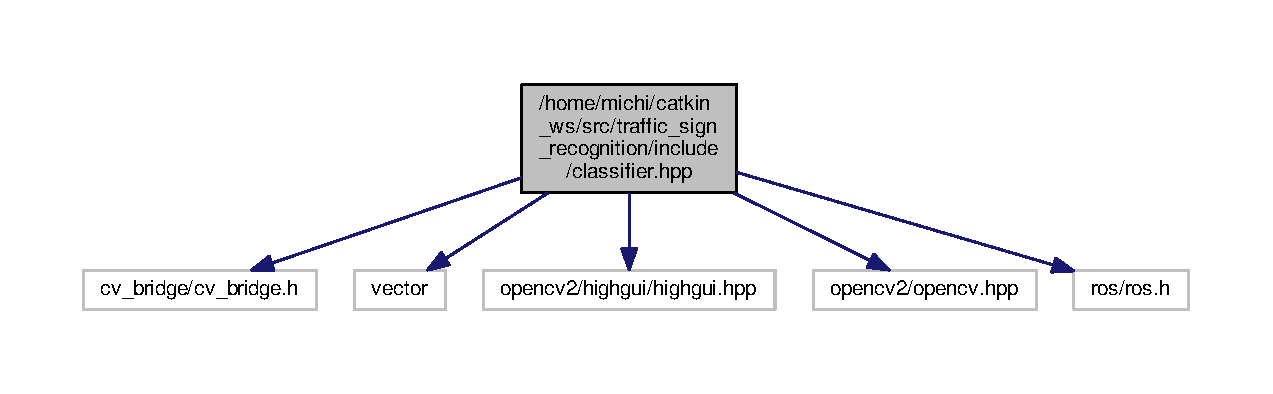
\includegraphics[width=350pt]{classifier_8hpp__incl}
\end{center}
\end{figure}
This graph shows which files directly or indirectly include this file\+:
\nopagebreak
\begin{figure}[H]
\begin{center}
\leavevmode
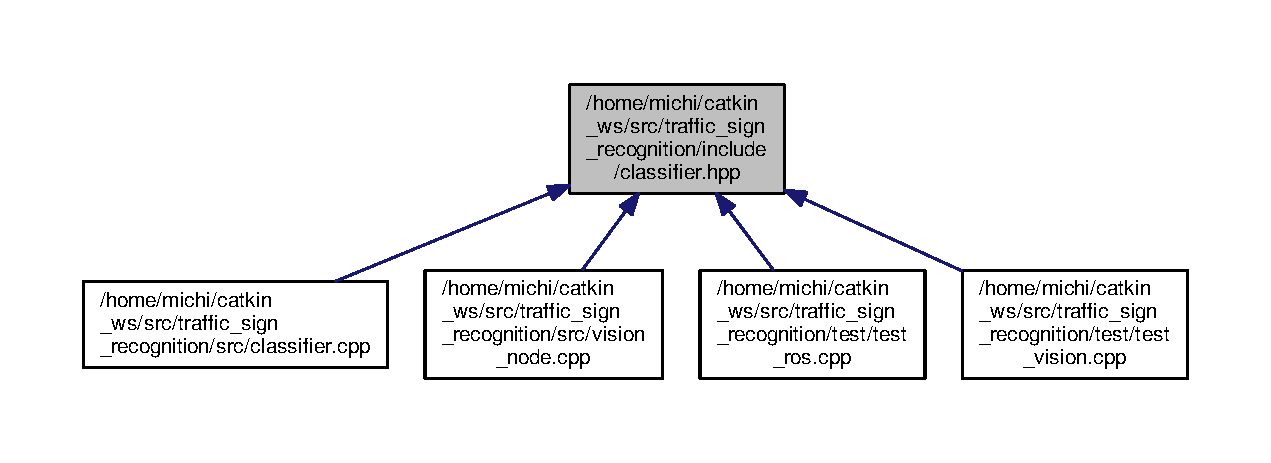
\includegraphics[width=350pt]{classifier_8hpp__dep__incl}
\end{center}
\end{figure}
\subsection*{Classes}
\begin{DoxyCompactItemize}
\item 
class \hyperlink{classclassifier}{classifier}
\begin{DoxyCompactList}\small\item\em Definition of the classifier class. It contains all the functions and variables depicted in the. \end{DoxyCompactList}\end{DoxyCompactItemize}


\subsection{Detailed Description}
Header file with definitions for class classifier. 

M\+IT License Copyright (c) 2017 Miguel Maestre Trueba Permission is hereby granted, free of charge, to any person obtaining a copy of this software and associated documentation files (the \char`\"{}\+Software\char`\"{}), to deal in the Software without restriction, including without limitation the rights to use, copy, modify, merge, publish, distribute, sublicense, and/or sell copies of the Software, and to permit persons to whom the Software is furnished to do so, subject to the following conditions\+: The above copyright notice and this permission notice shall be included in all copies or substantial portions of the Software. T\+HE S\+O\+F\+T\+W\+A\+RE IS P\+R\+O\+V\+I\+D\+ED \char`\"{}\+A\+S I\+S\char`\"{}, W\+I\+T\+H\+O\+UT W\+A\+R\+R\+A\+N\+TY OF A\+NY K\+I\+ND, E\+X\+P\+R\+E\+SS OR I\+M\+P\+L\+I\+ED, I\+N\+C\+L\+U\+D\+I\+NG B\+UT N\+OT L\+I\+M\+I\+T\+ED TO T\+HE W\+A\+R\+R\+A\+N\+T\+I\+ES OF M\+E\+R\+C\+H\+A\+N\+T\+A\+B\+I\+L\+I\+TY, F\+I\+T\+N\+E\+SS F\+OR A P\+A\+R\+T\+I\+C\+U\+L\+AR P\+U\+R\+P\+O\+SE A\+ND N\+O\+N\+I\+N\+F\+R\+I\+N\+G\+E\+M\+E\+NT. IN NO E\+V\+E\+NT S\+H\+A\+LL T\+HE A\+U\+T\+H\+O\+RS OR C\+O\+P\+Y\+R\+I\+G\+HT H\+O\+L\+D\+E\+RS BE L\+I\+A\+B\+LE F\+OR A\+NY C\+L\+A\+IM, D\+A\+M\+A\+G\+ES OR O\+T\+H\+ER L\+I\+A\+B\+I\+L\+I\+TY, W\+H\+E\+T\+H\+ER IN AN A\+C\+T\+I\+ON OF C\+O\+N\+T\+R\+A\+CT, T\+O\+RT OR O\+T\+H\+E\+R\+W\+I\+SE, A\+R\+I\+S\+I\+NG F\+R\+OM, O\+UT OF OR IN C\+O\+N\+N\+E\+C\+T\+I\+ON W\+I\+TH T\+HE S\+O\+F\+T\+W\+A\+RE OR T\+HE U\+SE OR O\+T\+H\+ER D\+E\+A\+L\+I\+N\+GS IN T\+HE S\+O\+F\+T\+W\+A\+RE.

\begin{DoxyCopyright}{Copyright}
Copyright 2017 Miguel Maestre Trueba
\end{DoxyCopyright}
\begin{DoxyAuthor}{Author}
Miguel Maestre Trueba 
\end{DoxyAuthor}

\hypertarget{robot_8hpp}{}\section{/home/michi/catkin\+\_\+ws/src/traffic\+\_\+sign\+\_\+recognition/include/robot.hpp File Reference}
\label{robot_8hpp}\index{/home/michi/catkin\+\_\+ws/src/traffic\+\_\+sign\+\_\+recognition/include/robot.\+hpp@{/home/michi/catkin\+\_\+ws/src/traffic\+\_\+sign\+\_\+recognition/include/robot.\+hpp}}


Header file with definitions for class robot.  


{\ttfamily \#include $<$geometry\+\_\+msgs/\+Twist.\+h$>$}\\*
{\ttfamily \#include $<$vector$>$}\\*
{\ttfamily \#include \char`\"{}ros/ros.\+h\char`\"{}}\\*
{\ttfamily \#include \char`\"{}traffic\+\_\+sign\+\_\+recognition/sign.\+h\char`\"{}}\\*
Include dependency graph for robot.\+hpp\+:
\nopagebreak
\begin{figure}[H]
\begin{center}
\leavevmode
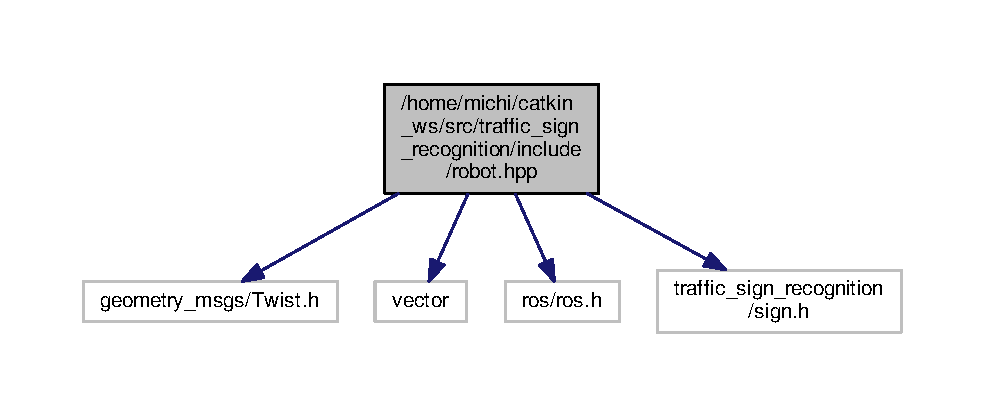
\includegraphics[width=350pt]{robot_8hpp__incl}
\end{center}
\end{figure}
This graph shows which files directly or indirectly include this file\+:
\nopagebreak
\begin{figure}[H]
\begin{center}
\leavevmode
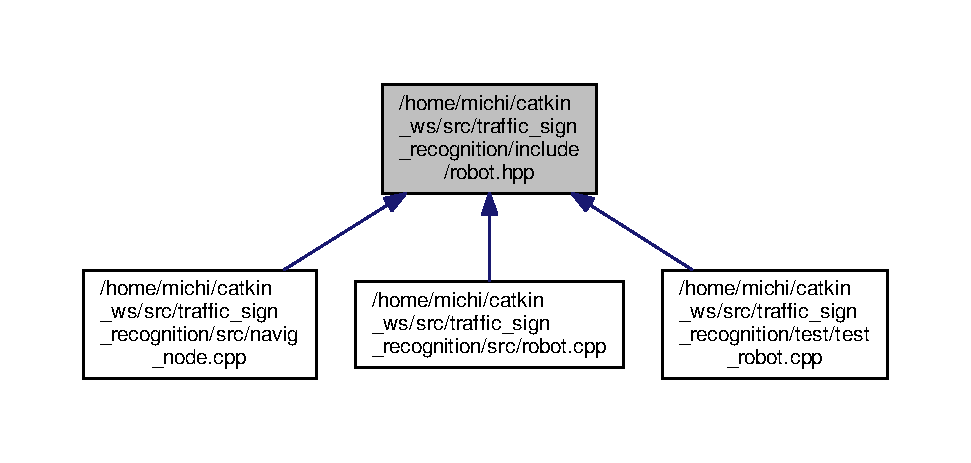
\includegraphics[width=350pt]{robot_8hpp__dep__incl}
\end{center}
\end{figure}
\subsection*{Classes}
\begin{DoxyCompactItemize}
\item 
class \hyperlink{classrobot}{robot}
\end{DoxyCompactItemize}


\subsection{Detailed Description}
Header file with definitions for class robot. 

M\+IT License Copyright (c) 2017 Miguel Maestre Trueba Permission is hereby granted, free of charge, to any person obtaining a copy of this software and associated documentation files (the \char`\"{}\+Software\char`\"{}), to deal in the Software without restriction, including without limitation the rights to use, copy, modify, merge, publish, distribute, sublicense, and/or sell copies of the Software, and to permit persons to whom the Software is furnished to do so, subject to the following conditions\+: The above copyright notice and this permission notice shall be included in all copies or substantial portions of the Software. T\+HE S\+O\+F\+T\+W\+A\+RE IS P\+R\+O\+V\+I\+D\+ED \char`\"{}\+A\+S I\+S\char`\"{}, W\+I\+T\+H\+O\+UT W\+A\+R\+R\+A\+N\+TY OF A\+NY K\+I\+ND, E\+X\+P\+R\+E\+SS OR I\+M\+P\+L\+I\+ED, I\+N\+C\+L\+U\+D\+I\+NG B\+UT N\+OT L\+I\+M\+I\+T\+ED TO T\+HE W\+A\+R\+R\+A\+N\+T\+I\+ES OF M\+E\+R\+C\+H\+A\+N\+T\+A\+B\+I\+L\+I\+TY, F\+I\+T\+N\+E\+SS F\+OR A P\+A\+R\+T\+I\+C\+U\+L\+AR P\+U\+R\+P\+O\+SE A\+ND N\+O\+N\+I\+N\+F\+R\+I\+N\+G\+E\+M\+E\+NT. IN NO E\+V\+E\+NT S\+H\+A\+LL T\+HE A\+U\+T\+H\+O\+RS OR C\+O\+P\+Y\+R\+I\+G\+HT H\+O\+L\+D\+E\+RS BE L\+I\+A\+B\+LE F\+OR A\+NY C\+L\+A\+IM, D\+A\+M\+A\+G\+ES OR O\+T\+H\+ER L\+I\+A\+B\+I\+L\+I\+TY, W\+H\+E\+T\+H\+ER IN AN A\+C\+T\+I\+ON OF C\+O\+N\+T\+R\+A\+CT, T\+O\+RT OR O\+T\+H\+E\+R\+W\+I\+SE, A\+R\+I\+S\+I\+NG F\+R\+OM, O\+UT OF OR IN C\+O\+N\+N\+E\+C\+T\+I\+ON W\+I\+TH T\+HE S\+O\+F\+T\+W\+A\+RE OR T\+HE U\+SE OR O\+T\+H\+ER D\+E\+A\+L\+I\+N\+GS IN T\+HE S\+O\+F\+T\+W\+A\+RE.

\begin{DoxyCopyright}{Copyright}
Copyright 2017 Miguel Maestre Trueba
\end{DoxyCopyright}
\begin{DoxyAuthor}{Author}
Miguel Maestre Trueba 
\end{DoxyAuthor}

\hypertarget{classifier_8cpp}{}\section{/home/michi/catkin\+\_\+ws/src/traffic\+\_\+sign\+\_\+recognition/src/classifier.cpp File Reference}
\label{classifier_8cpp}\index{/home/michi/catkin\+\_\+ws/src/traffic\+\_\+sign\+\_\+recognition/src/classifier.\+cpp@{/home/michi/catkin\+\_\+ws/src/traffic\+\_\+sign\+\_\+recognition/src/classifier.\+cpp}}


Implementation of the methods of class classifier.  


{\ttfamily \#include $<$cv\+\_\+bridge/cv\+\_\+bridge.\+h$>$}\\*
{\ttfamily \#include $<$cstdlib$>$}\\*
{\ttfamily \#include $<$string$>$}\\*
{\ttfamily \#include $<$opencv2/highgui/highgui.\+hpp$>$}\\*
{\ttfamily \#include \char`\"{}ros/ros.\+h\char`\"{}}\\*
{\ttfamily \#include \char`\"{}opencv2/opencv.\+hpp\char`\"{}}\\*
{\ttfamily \#include \char`\"{}ros/console.\+h\char`\"{}}\\*
{\ttfamily \#include \char`\"{}classifier.\+hpp\char`\"{}}\\*
Include dependency graph for classifier.\+cpp\+:
\nopagebreak
\begin{figure}[H]
\begin{center}
\leavevmode
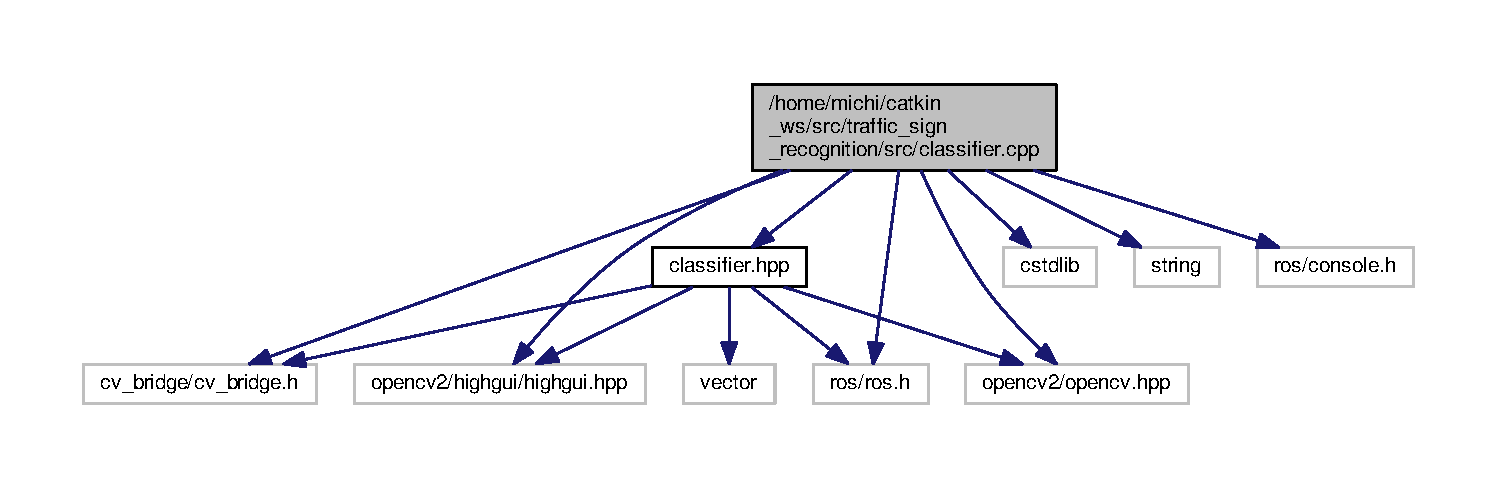
\includegraphics[width=350pt]{classifier_8cpp__incl}
\end{center}
\end{figure}


\subsection{Detailed Description}
Implementation of the methods of class classifier. 

M\+IT License Copyright (c) 2017 Miguel Maestre Trueba Permission is hereby granted, free of charge, to any person obtaining a copy of this software and associated documentation files (the \char`\"{}\+Software\char`\"{}), to deal in the Software without restriction, including without limitation the rights to use, copy, modify, merge, publish, distribute, sublicense, and/or sell copies of the Software, and to permit persons to whom the Software is furnished to do so, subject to the following conditions\+: The above copyright notice and this permission notice shall be included in all copies or substantial portions of the Software. T\+HE S\+O\+F\+T\+W\+A\+RE IS P\+R\+O\+V\+I\+D\+ED \char`\"{}\+A\+S I\+S\char`\"{}, W\+I\+T\+H\+O\+UT W\+A\+R\+R\+A\+N\+TY OF A\+NY K\+I\+ND, E\+X\+P\+R\+E\+SS OR I\+M\+P\+L\+I\+ED, I\+N\+C\+L\+U\+D\+I\+NG B\+UT N\+OT L\+I\+M\+I\+T\+ED TO T\+HE W\+A\+R\+R\+A\+N\+T\+I\+ES OF M\+E\+R\+C\+H\+A\+N\+T\+A\+B\+I\+L\+I\+TY, F\+I\+T\+N\+E\+SS F\+OR A P\+A\+R\+T\+I\+C\+U\+L\+AR P\+U\+R\+P\+O\+SE A\+ND N\+O\+N\+I\+N\+F\+R\+I\+N\+G\+E\+M\+E\+NT. IN NO E\+V\+E\+NT S\+H\+A\+LL T\+HE A\+U\+T\+H\+O\+RS OR C\+O\+P\+Y\+R\+I\+G\+HT H\+O\+L\+D\+E\+RS BE L\+I\+A\+B\+LE F\+OR A\+NY C\+L\+A\+IM, D\+A\+M\+A\+G\+ES OR O\+T\+H\+ER L\+I\+A\+B\+I\+L\+I\+TY, W\+H\+E\+T\+H\+ER IN AN A\+C\+T\+I\+ON OF C\+O\+N\+T\+R\+A\+CT, T\+O\+RT OR O\+T\+H\+E\+R\+W\+I\+SE, A\+R\+I\+S\+I\+NG F\+R\+OM, O\+UT OF OR IN C\+O\+N\+N\+E\+C\+T\+I\+ON W\+I\+TH T\+HE S\+O\+F\+T\+W\+A\+RE OR T\+HE U\+SE OR O\+T\+H\+ER D\+E\+A\+L\+I\+N\+GS IN T\+HE S\+O\+F\+T\+W\+A\+RE.

\begin{DoxyCopyright}{Copyright}
Copyright 2017 Miguel Maestre Trueba
\end{DoxyCopyright}
\begin{DoxyAuthor}{Author}
Miguel Maestre Trueba These methods are in charge of receiving images and detecting and classifying signs in the images. 
\end{DoxyAuthor}

\hypertarget{navig__node_8cpp}{}\section{/home/michi/catkin\+\_\+ws/src/traffic\+\_\+sign\+\_\+recognition/src/navig\+\_\+node.cpp File Reference}
\label{navig__node_8cpp}\index{/home/michi/catkin\+\_\+ws/src/traffic\+\_\+sign\+\_\+recognition/src/navig\+\_\+node.\+cpp@{/home/michi/catkin\+\_\+ws/src/traffic\+\_\+sign\+\_\+recognition/src/navig\+\_\+node.\+cpp}}


Navigation node where all the main functions of the robot behavious happen.  


{\ttfamily \#include $<$string$>$}\\*
{\ttfamily \#include $<$cstdlib$>$}\\*
{\ttfamily \#include \char`\"{}ros/ros.\+h\char`\"{}}\\*
{\ttfamily \#include \char`\"{}ros/console.\+h\char`\"{}}\\*
{\ttfamily \#include \char`\"{}robot.\+hpp\char`\"{}}\\*
{\ttfamily \#include \char`\"{}traffic\+\_\+sign\+\_\+recognition/sign.\+h\char`\"{}}\\*
Include dependency graph for navig\+\_\+node.\+cpp\+:
\nopagebreak
\begin{figure}[H]
\begin{center}
\leavevmode
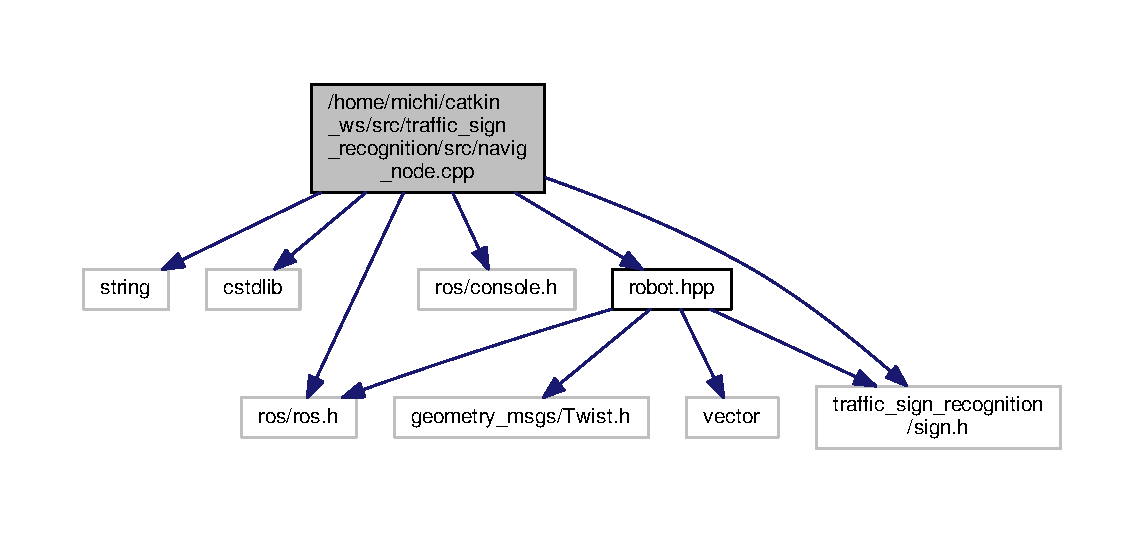
\includegraphics[width=350pt]{navig__node_8cpp__incl}
\end{center}
\end{figure}
\subsection*{Functions}
\begin{DoxyCompactItemize}
\item 
int \hyperlink{navig__node_8cpp_a3c04138a5bfe5d72780bb7e82a18e627}{main} (int argc, char $\ast$$\ast$argv)
\begin{DoxyCompactList}\small\item\em Function main that runs the main algorithm of the robot behavior. \end{DoxyCompactList}\end{DoxyCompactItemize}


\subsection{Detailed Description}
Navigation node where all the main functions of the robot behavious happen. 

M\+IT License Copyright (c) 2017 Miguel Maestre Trueba Permission is hereby granted, free of charge, to any person obtaining a copy of this software and associated documentation files (the \char`\"{}\+Software\char`\"{}), to deal in the Software without restriction, including without limitation the rights to use, copy, modify, merge, publish, distribute, sublicense, and/or sell copies of the Software, and to permit persons to whom the Software is furnished to do so, subject to the following conditions\+: The above copyright notice and this permission notice shall be included in all copies or substantial portions of the Software. T\+HE S\+O\+F\+T\+W\+A\+RE IS P\+R\+O\+V\+I\+D\+ED \char`\"{}\+A\+S I\+S\char`\"{}, W\+I\+T\+H\+O\+UT W\+A\+R\+R\+A\+N\+TY OF A\+NY K\+I\+ND, E\+X\+P\+R\+E\+SS OR I\+M\+P\+L\+I\+ED, I\+N\+C\+L\+U\+D\+I\+NG B\+UT N\+OT L\+I\+M\+I\+T\+ED TO T\+HE W\+A\+R\+R\+A\+N\+T\+I\+ES OF M\+E\+R\+C\+H\+A\+N\+T\+A\+B\+I\+L\+I\+TY, F\+I\+T\+N\+E\+SS F\+OR A P\+A\+R\+T\+I\+C\+U\+L\+AR P\+U\+R\+P\+O\+SE A\+ND N\+O\+N\+I\+N\+F\+R\+I\+N\+G\+E\+M\+E\+NT. IN NO E\+V\+E\+NT S\+H\+A\+LL T\+HE A\+U\+T\+H\+O\+RS OR C\+O\+P\+Y\+R\+I\+G\+HT H\+O\+L\+D\+E\+RS BE L\+I\+A\+B\+LE F\+OR A\+NY C\+L\+A\+IM, D\+A\+M\+A\+G\+ES OR O\+T\+H\+ER L\+I\+A\+B\+I\+L\+I\+TY, W\+H\+E\+T\+H\+ER IN AN A\+C\+T\+I\+ON OF C\+O\+N\+T\+R\+A\+CT, T\+O\+RT OR O\+T\+H\+E\+R\+W\+I\+SE, A\+R\+I\+S\+I\+NG F\+R\+OM, O\+UT OF OR IN C\+O\+N\+N\+E\+C\+T\+I\+ON W\+I\+TH T\+HE S\+O\+F\+T\+W\+A\+RE OR T\+HE U\+SE OR O\+T\+H\+ER D\+E\+A\+L\+I\+N\+GS IN T\+HE S\+O\+F\+T\+W\+A\+RE.

\begin{DoxyCopyright}{Copyright}
Copyright 2017 Miguel Maestre Trueba
\end{DoxyCopyright}
\begin{DoxyAuthor}{Author}
Miguel Maestre Trueba 
\end{DoxyAuthor}


\subsection{Function Documentation}
\index{navig\+\_\+node.\+cpp@{navig\+\_\+node.\+cpp}!main@{main}}
\index{main@{main}!navig\+\_\+node.\+cpp@{navig\+\_\+node.\+cpp}}
\subsubsection[{\texorpdfstring{main(int argc, char $\ast$$\ast$argv)}{main(int argc, char **argv)}}]{\setlength{\rightskip}{0pt plus 5cm}int main (
\begin{DoxyParamCaption}
\item[{int}]{argc, }
\item[{char $\ast$$\ast$}]{argv}
\end{DoxyParamCaption}
)}\hypertarget{navig__node_8cpp_a3c04138a5bfe5d72780bb7e82a18e627}{}\label{navig__node_8cpp_a3c04138a5bfe5d72780bb7e82a18e627}


Function main that runs the main algorithm of the robot behavior. 

It reads the messages published by the vision node using a R\+OS subscriber. Depending on what type of sign has been recognized, different actions will be executed. When the area of the detection is big enough and the sign classified, publish Twist messages to the robot. 
\begin{DoxyParams}{Parameters}
{\em argc} & is the number of arguments. \\
\hline
{\em argv} & is the arguments characters array. \\
\hline
\end{DoxyParams}
\begin{DoxyReturn}{Returns}
0 
\end{DoxyReturn}

\hypertarget{robot_8cpp}{}\section{/home/michi/catkin\+\_\+ws/src/traffic\+\_\+sign\+\_\+recognition/src/robot.cpp File Reference}
\label{robot_8cpp}\index{/home/michi/catkin\+\_\+ws/src/traffic\+\_\+sign\+\_\+recognition/src/robot.\+cpp@{/home/michi/catkin\+\_\+ws/src/traffic\+\_\+sign\+\_\+recognition/src/robot.\+cpp}}


Implementation of the methods of class robot.  


{\ttfamily \#include $<$geometry\+\_\+msgs/\+Twist.\+h$>$}\\*
{\ttfamily \#include $<$vector$>$}\\*
{\ttfamily \#include \char`\"{}ros/ros.\+h\char`\"{}}\\*
{\ttfamily \#include \char`\"{}ros/console.\+h\char`\"{}}\\*
{\ttfamily \#include \char`\"{}robot.\+hpp\char`\"{}}\\*
{\ttfamily \#include \char`\"{}traffic\+\_\+sign\+\_\+recognition/sign.\+h\char`\"{}}\\*
Include dependency graph for robot.\+cpp\+:
\nopagebreak
\begin{figure}[H]
\begin{center}
\leavevmode
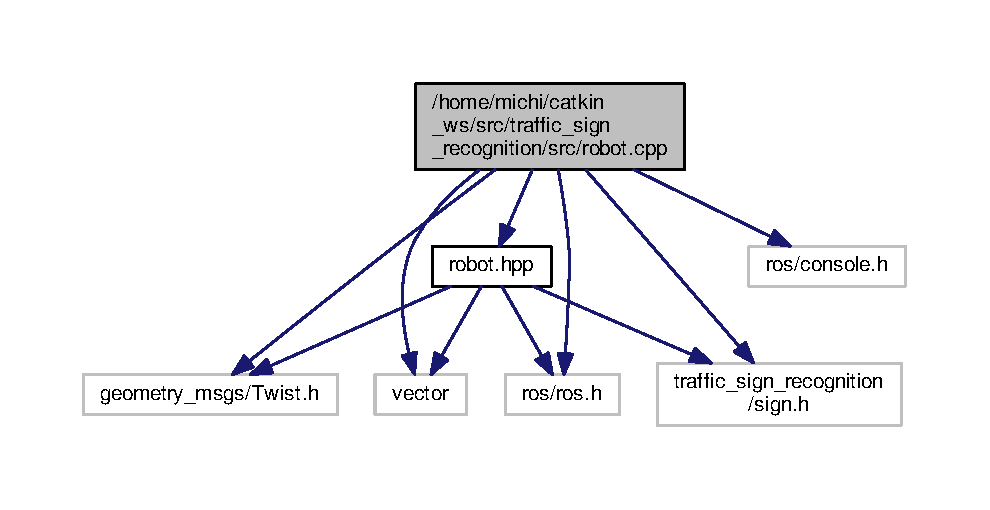
\includegraphics[width=350pt]{robot_8cpp__incl}
\end{center}
\end{figure}


\subsection{Detailed Description}
Implementation of the methods of class robot. 

M\+IT License Copyright (c) 2017 Miguel Maestre Trueba Permission is hereby granted, free of charge, to any person obtaining a copy of this software and associated documentation files (the \char`\"{}\+Software\char`\"{}), to deal in the Software without restriction, including without limitation the rights to use, copy, modify, merge, publish, distribute, sublicense, and/or sell copies of the Software, and to permit persons to whom the Software is furnished to do so, subject to the following conditions\+: The above copyright notice and this permission notice shall be included in all copies or substantial portions of the Software. T\+HE S\+O\+F\+T\+W\+A\+RE IS P\+R\+O\+V\+I\+D\+ED \char`\"{}\+A\+S I\+S\char`\"{}, W\+I\+T\+H\+O\+UT W\+A\+R\+R\+A\+N\+TY OF A\+NY K\+I\+ND, E\+X\+P\+R\+E\+SS OR I\+M\+P\+L\+I\+ED, I\+N\+C\+L\+U\+D\+I\+NG B\+UT N\+OT L\+I\+M\+I\+T\+ED TO T\+HE W\+A\+R\+R\+A\+N\+T\+I\+ES OF M\+E\+R\+C\+H\+A\+N\+T\+A\+B\+I\+L\+I\+TY, F\+I\+T\+N\+E\+SS F\+OR A P\+A\+R\+T\+I\+C\+U\+L\+AR P\+U\+R\+P\+O\+SE A\+ND N\+O\+N\+I\+N\+F\+R\+I\+N\+G\+E\+M\+E\+NT. IN NO E\+V\+E\+NT S\+H\+A\+LL T\+HE A\+U\+T\+H\+O\+RS OR C\+O\+P\+Y\+R\+I\+G\+HT H\+O\+L\+D\+E\+RS BE L\+I\+A\+B\+LE F\+OR A\+NY C\+L\+A\+IM, D\+A\+M\+A\+G\+ES OR O\+T\+H\+ER L\+I\+A\+B\+I\+L\+I\+TY, W\+H\+E\+T\+H\+ER IN AN A\+C\+T\+I\+ON OF C\+O\+N\+T\+R\+A\+CT, T\+O\+RT OR O\+T\+H\+E\+R\+W\+I\+SE, A\+R\+I\+S\+I\+NG F\+R\+OM, O\+UT OF OR IN C\+O\+N\+N\+E\+C\+T\+I\+ON W\+I\+TH T\+HE S\+O\+F\+T\+W\+A\+RE OR T\+HE U\+SE OR O\+T\+H\+ER D\+E\+A\+L\+I\+N\+GS IN T\+HE S\+O\+F\+T\+W\+A\+RE.

\begin{DoxyCopyright}{Copyright}
Copyright 2017 Miguel Maestre Trueba
\end{DoxyCopyright}
\begin{DoxyAuthor}{Author}
Miguel Maestre Trueba These methods are in charge of receiving messages and moving the robot depending on the information of the msg. 
\end{DoxyAuthor}

\hypertarget{vision__node_8cpp}{}\section{/home/michi/catkin\+\_\+ws/src/traffic\+\_\+sign\+\_\+recognition/src/vision\+\_\+node.cpp File Reference}
\label{vision__node_8cpp}\index{/home/michi/catkin\+\_\+ws/src/traffic\+\_\+sign\+\_\+recognition/src/vision\+\_\+node.\+cpp@{/home/michi/catkin\+\_\+ws/src/traffic\+\_\+sign\+\_\+recognition/src/vision\+\_\+node.\+cpp}}


Vision node where all the main functions of the detection and recognition happen.  


{\ttfamily \#include $<$cv\+\_\+bridge/cv\+\_\+bridge.\+h$>$}\\*
{\ttfamily \#include $<$cstdlib$>$}\\*
{\ttfamily \#include $<$string$>$}\\*
{\ttfamily \#include $<$opencv2/highgui/highgui.\+hpp$>$}\\*
{\ttfamily \#include \char`\"{}opencv2/opencv.\+hpp\char`\"{}}\\*
{\ttfamily \#include \char`\"{}ros/ros.\+h\char`\"{}}\\*
{\ttfamily \#include \char`\"{}ros/console.\+h\char`\"{}}\\*
{\ttfamily \#include \char`\"{}classifier.\+hpp\char`\"{}}\\*
{\ttfamily \#include \char`\"{}traffic\+\_\+sign\+\_\+recognition/sign.\+h\char`\"{}}\\*
Include dependency graph for vision\+\_\+node.\+cpp\+:
\nopagebreak
\begin{figure}[H]
\begin{center}
\leavevmode
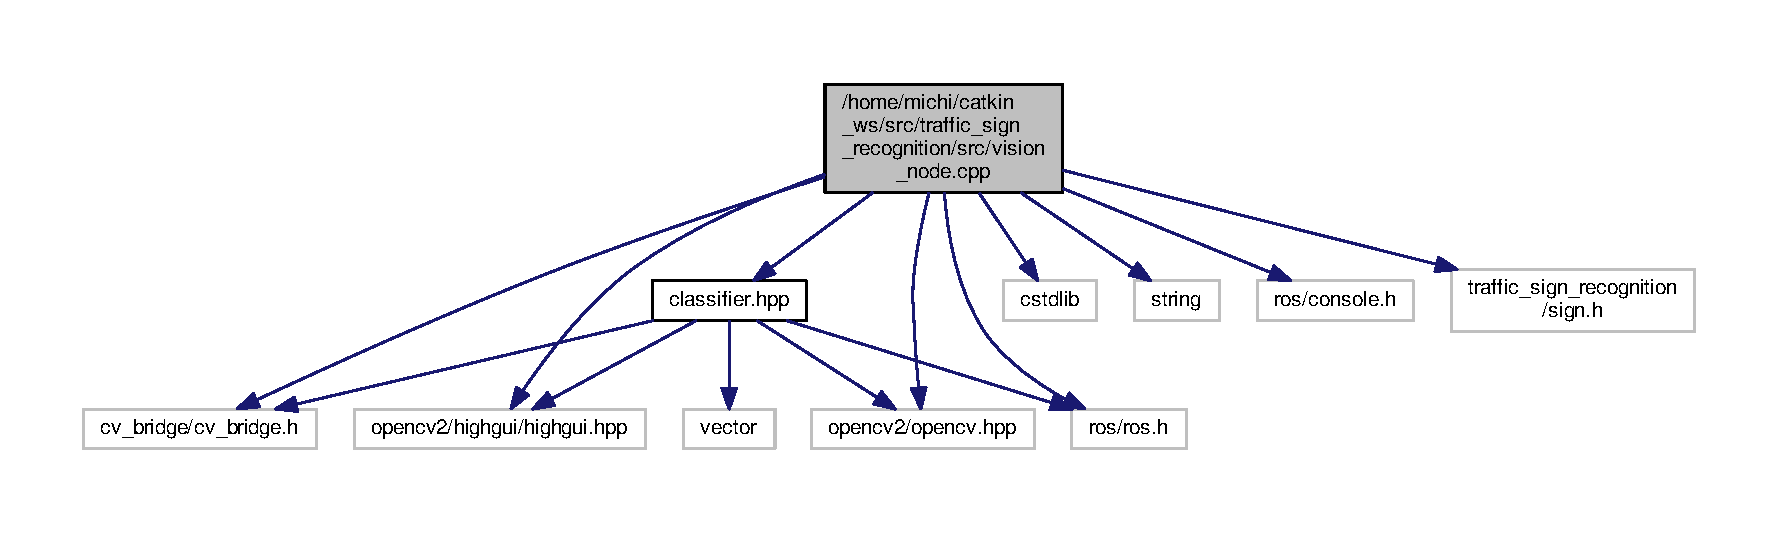
\includegraphics[width=350pt]{vision__node_8cpp__incl}
\end{center}
\end{figure}
\subsection*{Functions}
\begin{DoxyCompactItemize}
\item 
int \hyperlink{vision__node_8cpp_a3c04138a5bfe5d72780bb7e82a18e627}{main} (int argc, char $\ast$$\ast$argv)
\begin{DoxyCompactList}\small\item\em Function main that runs the main algorithm of the traffic sign recognition. \end{DoxyCompactList}\end{DoxyCompactItemize}


\subsection{Detailed Description}
Vision node where all the main functions of the detection and recognition happen. 

M\+IT License Copyright (c) 2017 Miguel Maestre Trueba Permission is hereby granted, free of charge, to any person obtaining a copy of this software and associated documentation files (the \char`\"{}\+Software\char`\"{}), to deal in the Software without restriction, including without limitation the rights to use, copy, modify, merge, publish, distribute, sublicense, and/or sell copies of the Software, and to permit persons to whom the Software is furnished to do so, subject to the following conditions\+: The above copyright notice and this permission notice shall be included in all copies or substantial portions of the Software. T\+HE S\+O\+F\+T\+W\+A\+RE IS P\+R\+O\+V\+I\+D\+ED \char`\"{}\+A\+S I\+S\char`\"{}, W\+I\+T\+H\+O\+UT W\+A\+R\+R\+A\+N\+TY OF A\+NY K\+I\+ND, E\+X\+P\+R\+E\+SS OR I\+M\+P\+L\+I\+ED, I\+N\+C\+L\+U\+D\+I\+NG B\+UT N\+OT L\+I\+M\+I\+T\+ED TO T\+HE W\+A\+R\+R\+A\+N\+T\+I\+ES OF M\+E\+R\+C\+H\+A\+N\+T\+A\+B\+I\+L\+I\+TY, F\+I\+T\+N\+E\+SS F\+OR A P\+A\+R\+T\+I\+C\+U\+L\+AR P\+U\+R\+P\+O\+SE A\+ND N\+O\+N\+I\+N\+F\+R\+I\+N\+G\+E\+M\+E\+NT. IN NO E\+V\+E\+NT S\+H\+A\+LL T\+HE A\+U\+T\+H\+O\+RS OR C\+O\+P\+Y\+R\+I\+G\+HT H\+O\+L\+D\+E\+RS BE L\+I\+A\+B\+LE F\+OR A\+NY C\+L\+A\+IM, D\+A\+M\+A\+G\+ES OR O\+T\+H\+ER L\+I\+A\+B\+I\+L\+I\+TY, W\+H\+E\+T\+H\+ER IN AN A\+C\+T\+I\+ON OF C\+O\+N\+T\+R\+A\+CT, T\+O\+RT OR O\+T\+H\+E\+R\+W\+I\+SE, A\+R\+I\+S\+I\+NG F\+R\+OM, O\+UT OF OR IN C\+O\+N\+N\+E\+C\+T\+I\+ON W\+I\+TH T\+HE S\+O\+F\+T\+W\+A\+RE OR T\+HE U\+SE OR O\+T\+H\+ER D\+E\+A\+L\+I\+N\+GS IN T\+HE S\+O\+F\+T\+W\+A\+RE.

\begin{DoxyCopyright}{Copyright}
Copyright 2017 Miguel Maestre Trueba
\end{DoxyCopyright}
\begin{DoxyAuthor}{Author}
Miguel Maestre Trueba 
\end{DoxyAuthor}


\subsection{Function Documentation}
\index{vision\+\_\+node.\+cpp@{vision\+\_\+node.\+cpp}!main@{main}}
\index{main@{main}!vision\+\_\+node.\+cpp@{vision\+\_\+node.\+cpp}}
\subsubsection[{\texorpdfstring{main(int argc, char $\ast$$\ast$argv)}{main(int argc, char **argv)}}]{\setlength{\rightskip}{0pt plus 5cm}int main (
\begin{DoxyParamCaption}
\item[{int}]{argc, }
\item[{char $\ast$$\ast$}]{argv}
\end{DoxyParamCaption}
)}\hypertarget{vision__node_8cpp_a3c04138a5bfe5d72780bb7e82a18e627}{}\label{vision__node_8cpp_a3c04138a5bfe5d72780bb7e82a18e627}


Function main that runs the main algorithm of the traffic sign recognition. 

It reads images from the robot\textquotesingle{}s camera using a R\+OS subscriber. A S\+VM is trained and used to classify new signs features found by the robot. The type of sign and the size of the detection are published using a custom message. 
\begin{DoxyParams}{Parameters}
{\em argc} & is the number of arguments. \\
\hline
{\em argv} & is the arguments characters array. \\
\hline
\end{DoxyParams}
\begin{DoxyReturn}{Returns}
0 
\end{DoxyReturn}

\hypertarget{test__robot_8cpp}{}\section{/home/michi/catkin\+\_\+ws/src/traffic\+\_\+sign\+\_\+recognition/test/test\+\_\+robot.cpp File Reference}
\label{test__robot_8cpp}\index{/home/michi/catkin\+\_\+ws/src/traffic\+\_\+sign\+\_\+recognition/test/test\+\_\+robot.\+cpp@{/home/michi/catkin\+\_\+ws/src/traffic\+\_\+sign\+\_\+recognition/test/test\+\_\+robot.\+cpp}}


Unit test code for class robot.  


{\ttfamily \#include $<$gtest/gtest.\+h$>$}\\*
{\ttfamily \#include $<$vector$>$}\\*
{\ttfamily \#include \char`\"{}ros/ros.\+h\char`\"{}}\\*
{\ttfamily \#include \char`\"{}robot.\+hpp\char`\"{}}\\*
{\ttfamily \#include \char`\"{}traffic\+\_\+sign\+\_\+recognition/sign.\+h\char`\"{}}\\*
Include dependency graph for test\+\_\+robot.\+cpp\+:
\nopagebreak
\begin{figure}[H]
\begin{center}
\leavevmode
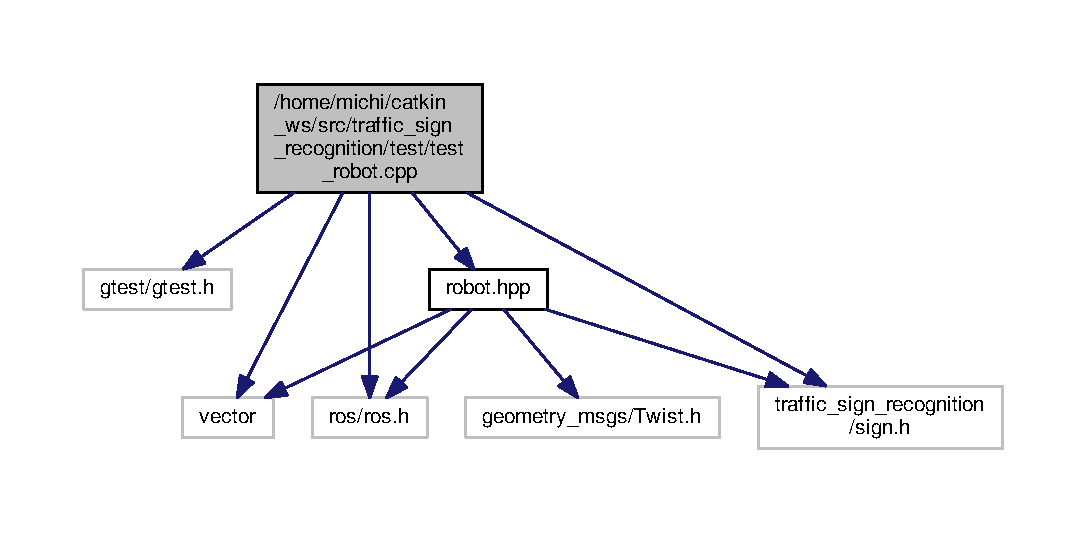
\includegraphics[width=350pt]{test__robot_8cpp__incl}
\end{center}
\end{figure}
\subsection*{Functions}
\begin{DoxyCompactItemize}
\item 
bool \hyperlink{test__robot_8cpp_a0410823cb65689901d9050a33298d6f6}{testing\+\_\+moves} (float sign\+\_\+type, double Area, bool Flag)
\begin{DoxyCompactList}\small\item\em Function that simulates velocity commands depending on the input. \end{DoxyCompactList}\item 
float \hyperlink{test__robot_8cpp_a67c4f477c5750177da5e0b00b8aca6de}{test\+\_\+callback} (double Area)
\begin{DoxyCompactList}\small\item\em Function that tests the sign message callback. \end{DoxyCompactList}\item 
\hyperlink{test__robot_8cpp_a1b95106f12f1122945e42b275f3fc29e}{T\+E\+ST} (Test\+Command, Forward\+Test)
\begin{DoxyCompactList}\small\item\em Test if robot publishes the right command when forward sign detected. \end{DoxyCompactList}\item 
\hyperlink{test__robot_8cpp_a0b3a3335108f4fb2c5e3870f06db72fa}{T\+E\+ST} (Test\+Command, Turn\+Test)
\begin{DoxyCompactList}\small\item\em Test if robot publishes the right command when turn sign detected. \end{DoxyCompactList}\item 
\hyperlink{test__robot_8cpp_a3557ae93eb9a3c4c6b386ae8f9519a79}{T\+E\+ST} (Test\+Command, Stop\+Test)
\begin{DoxyCompactList}\small\item\em Test if robot publishes the right command when stop sign detected. \end{DoxyCompactList}\item 
\hyperlink{test__robot_8cpp_a9af05c96a743a738946dc6dd8142d14b}{T\+E\+ST} (Test\+Command, Callback\+Test)
\begin{DoxyCompactList}\small\item\em Test if callback stores correctly different types of area inputs. \end{DoxyCompactList}\item 
int \hyperlink{test__robot_8cpp_a3c04138a5bfe5d72780bb7e82a18e627}{main} (int argc, char $\ast$$\ast$argv)
\begin{DoxyCompactList}\small\item\em Main function that runs all tests in the file. \end{DoxyCompactList}\end{DoxyCompactItemize}


\subsection{Detailed Description}
Unit test code for class robot. 

M\+IT License Copyright (c) 2017 Miguel Maestre Trueba Permission is hereby granted, free of charge, to any person obtaining a copy of this software and associated documentation files (the \char`\"{}\+Software\char`\"{}), to deal in the Software without restriction, including without limitation the rights to use, copy, modify, merge, publish, distribute, sublicense, and/or sell copies of the Software, and to permit persons to whom the Software is furnished to do so, subject to the following conditions\+: The above copyright notice and this permission notice shall be included in all copies or substantial portions of the Software. T\+HE S\+O\+F\+T\+W\+A\+RE IS P\+R\+O\+V\+I\+D\+ED \char`\"{}\+A\+S I\+S\char`\"{}, W\+I\+T\+H\+O\+UT W\+A\+R\+R\+A\+N\+TY OF A\+NY K\+I\+ND, E\+X\+P\+R\+E\+SS OR I\+M\+P\+L\+I\+ED, I\+N\+C\+L\+U\+D\+I\+NG B\+UT N\+OT L\+I\+M\+I\+T\+ED TO T\+HE W\+A\+R\+R\+A\+N\+T\+I\+ES OF M\+E\+R\+C\+H\+A\+N\+T\+A\+B\+I\+L\+I\+TY, F\+I\+T\+N\+E\+SS F\+OR A P\+A\+R\+T\+I\+C\+U\+L\+AR P\+U\+R\+P\+O\+SE A\+ND N\+O\+N\+I\+N\+F\+R\+I\+N\+G\+E\+M\+E\+NT. IN NO E\+V\+E\+NT S\+H\+A\+LL T\+HE A\+U\+T\+H\+O\+RS OR C\+O\+P\+Y\+R\+I\+G\+HT H\+O\+L\+D\+E\+RS BE L\+I\+A\+B\+LE F\+OR A\+NY C\+L\+A\+IM, D\+A\+M\+A\+G\+ES OR O\+T\+H\+ER L\+I\+A\+B\+I\+L\+I\+TY, W\+H\+E\+T\+H\+ER IN AN A\+C\+T\+I\+ON OF C\+O\+N\+T\+R\+A\+CT, T\+O\+RT OR O\+T\+H\+E\+R\+W\+I\+SE, A\+R\+I\+S\+I\+NG F\+R\+OM, O\+UT OF OR IN C\+O\+N\+N\+E\+C\+T\+I\+ON W\+I\+TH T\+HE S\+O\+F\+T\+W\+A\+RE OR T\+HE U\+SE OR O\+T\+H\+ER D\+E\+A\+L\+I\+N\+GS IN T\+HE S\+O\+F\+T\+W\+A\+RE.

\begin{DoxyCopyright}{Copyright}
Copyright 2017 Miguel Maestre Trueba
\end{DoxyCopyright}
\begin{DoxyAuthor}{Author}
Miguel Maestre Trueba 
\end{DoxyAuthor}


\subsection{Function Documentation}
\index{test\+\_\+robot.\+cpp@{test\+\_\+robot.\+cpp}!main@{main}}
\index{main@{main}!test\+\_\+robot.\+cpp@{test\+\_\+robot.\+cpp}}
\subsubsection[{\texorpdfstring{main(int argc, char $\ast$$\ast$argv)}{main(int argc, char **argv)}}]{\setlength{\rightskip}{0pt plus 5cm}int main (
\begin{DoxyParamCaption}
\item[{int}]{argc, }
\item[{char $\ast$$\ast$}]{argv}
\end{DoxyParamCaption}
)}\hypertarget{test__robot_8cpp_a3c04138a5bfe5d72780bb7e82a18e627}{}\label{test__robot_8cpp_a3c04138a5bfe5d72780bb7e82a18e627}


Main function that runs all tests in the file. 


\begin{DoxyParams}{Parameters}
{\em argc} & is the number of arguments \\
\hline
{\em argv} & is the arguments characters array \\
\hline
\end{DoxyParams}
\begin{DoxyReturn}{Returns}
Tests results 
\end{DoxyReturn}
\index{test\+\_\+robot.\+cpp@{test\+\_\+robot.\+cpp}!T\+E\+ST@{T\+E\+ST}}
\index{T\+E\+ST@{T\+E\+ST}!test\+\_\+robot.\+cpp@{test\+\_\+robot.\+cpp}}
\subsubsection[{\texorpdfstring{T\+E\+S\+T(\+Test\+Command, Forward\+Test)}{TEST(TestCommand, ForwardTest)}}]{\setlength{\rightskip}{0pt plus 5cm}T\+E\+ST (
\begin{DoxyParamCaption}
\item[{Test\+Command}]{, }
\item[{Forward\+Test}]{}
\end{DoxyParamCaption}
)}\hypertarget{test__robot_8cpp_a1b95106f12f1122945e42b275f3fc29e}{}\label{test__robot_8cpp_a1b95106f12f1122945e42b275f3fc29e}


Test if robot publishes the right command when forward sign detected. 


\begin{DoxyParams}{Parameters}
{\em none} & \\
\hline
\end{DoxyParams}
\begin{DoxyReturn}{Returns}
none 
\end{DoxyReturn}
\index{test\+\_\+robot.\+cpp@{test\+\_\+robot.\+cpp}!T\+E\+ST@{T\+E\+ST}}
\index{T\+E\+ST@{T\+E\+ST}!test\+\_\+robot.\+cpp@{test\+\_\+robot.\+cpp}}
\subsubsection[{\texorpdfstring{T\+E\+S\+T(\+Test\+Command, Turn\+Test)}{TEST(TestCommand, TurnTest)}}]{\setlength{\rightskip}{0pt plus 5cm}T\+E\+ST (
\begin{DoxyParamCaption}
\item[{Test\+Command}]{, }
\item[{Turn\+Test}]{}
\end{DoxyParamCaption}
)}\hypertarget{test__robot_8cpp_a0b3a3335108f4fb2c5e3870f06db72fa}{}\label{test__robot_8cpp_a0b3a3335108f4fb2c5e3870f06db72fa}


Test if robot publishes the right command when turn sign detected. 


\begin{DoxyParams}{Parameters}
{\em none} & \\
\hline
\end{DoxyParams}
\begin{DoxyReturn}{Returns}
none 
\end{DoxyReturn}
\index{test\+\_\+robot.\+cpp@{test\+\_\+robot.\+cpp}!T\+E\+ST@{T\+E\+ST}}
\index{T\+E\+ST@{T\+E\+ST}!test\+\_\+robot.\+cpp@{test\+\_\+robot.\+cpp}}
\subsubsection[{\texorpdfstring{T\+E\+S\+T(\+Test\+Command, Stop\+Test)}{TEST(TestCommand, StopTest)}}]{\setlength{\rightskip}{0pt plus 5cm}T\+E\+ST (
\begin{DoxyParamCaption}
\item[{Test\+Command}]{, }
\item[{Stop\+Test}]{}
\end{DoxyParamCaption}
)}\hypertarget{test__robot_8cpp_a3557ae93eb9a3c4c6b386ae8f9519a79}{}\label{test__robot_8cpp_a3557ae93eb9a3c4c6b386ae8f9519a79}


Test if robot publishes the right command when stop sign detected. 


\begin{DoxyParams}{Parameters}
{\em none} & \\
\hline
\end{DoxyParams}
\begin{DoxyReturn}{Returns}
none 
\end{DoxyReturn}
\index{test\+\_\+robot.\+cpp@{test\+\_\+robot.\+cpp}!T\+E\+ST@{T\+E\+ST}}
\index{T\+E\+ST@{T\+E\+ST}!test\+\_\+robot.\+cpp@{test\+\_\+robot.\+cpp}}
\subsubsection[{\texorpdfstring{T\+E\+S\+T(\+Test\+Command, Callback\+Test)}{TEST(TestCommand, CallbackTest)}}]{\setlength{\rightskip}{0pt plus 5cm}T\+E\+ST (
\begin{DoxyParamCaption}
\item[{Test\+Command}]{, }
\item[{Callback\+Test}]{}
\end{DoxyParamCaption}
)}\hypertarget{test__robot_8cpp_a9af05c96a743a738946dc6dd8142d14b}{}\label{test__robot_8cpp_a9af05c96a743a738946dc6dd8142d14b}


Test if callback stores correctly different types of area inputs. 


\begin{DoxyParams}{Parameters}
{\em none} & \\
\hline
\end{DoxyParams}
\begin{DoxyReturn}{Returns}
none 
\end{DoxyReturn}
\index{test\+\_\+robot.\+cpp@{test\+\_\+robot.\+cpp}!test\+\_\+callback@{test\+\_\+callback}}
\index{test\+\_\+callback@{test\+\_\+callback}!test\+\_\+robot.\+cpp@{test\+\_\+robot.\+cpp}}
\subsubsection[{\texorpdfstring{test\+\_\+callback(double Area)}{test_callback(double Area)}}]{\setlength{\rightskip}{0pt plus 5cm}float test\+\_\+callback (
\begin{DoxyParamCaption}
\item[{double}]{Area}
\end{DoxyParamCaption}
)}\hypertarget{test__robot_8cpp_a67c4f477c5750177da5e0b00b8aca6de}{}\label{test__robot_8cpp_a67c4f477c5750177da5e0b00b8aca6de}


Function that tests the sign message callback. 


\begin{DoxyParams}{Parameters}
{\em Area} & is the area of the detections \\
\hline
\end{DoxyParams}
\begin{DoxyReturn}{Returns}
Returns the stored area if success 
\end{DoxyReturn}
\index{test\+\_\+robot.\+cpp@{test\+\_\+robot.\+cpp}!testing\+\_\+moves@{testing\+\_\+moves}}
\index{testing\+\_\+moves@{testing\+\_\+moves}!test\+\_\+robot.\+cpp@{test\+\_\+robot.\+cpp}}
\subsubsection[{\texorpdfstring{testing\+\_\+moves(float sign\+\_\+type, double Area, bool Flag)}{testing_moves(float sign_type, double Area, bool Flag)}}]{\setlength{\rightskip}{0pt plus 5cm}bool testing\+\_\+moves (
\begin{DoxyParamCaption}
\item[{float}]{sign\+\_\+type, }
\item[{double}]{Area, }
\item[{bool}]{Flag}
\end{DoxyParamCaption}
)}\hypertarget{test__robot_8cpp_a0410823cb65689901d9050a33298d6f6}{}\label{test__robot_8cpp_a0410823cb65689901d9050a33298d6f6}


Function that simulates velocity commands depending on the input. 


\begin{DoxyParams}{Parameters}
{\em sign\+\_\+type} & is the type of traffic sign detected \\
\hline
{\em Area} & is the area of the detected sign \\
\hline
{\em Flag} & is signal that activates the publishing of velocity \\
\hline
\end{DoxyParams}
\begin{DoxyReturn}{Returns}
Flag if succeeded 
\end{DoxyReturn}

\hypertarget{test__ros_8cpp}{}\section{/home/michi/catkin\+\_\+ws/src/traffic\+\_\+sign\+\_\+recognition/test/test\+\_\+ros.cpp File Reference}
\label{test__ros_8cpp}\index{/home/michi/catkin\+\_\+ws/src/traffic\+\_\+sign\+\_\+recognition/test/test\+\_\+ros.\+cpp@{/home/michi/catkin\+\_\+ws/src/traffic\+\_\+sign\+\_\+recognition/test/test\+\_\+ros.\+cpp}}


Unit tests for publishers and subscribers.  


{\ttfamily \#include $<$geometry\+\_\+msgs/\+Twist.\+h$>$}\\*
{\ttfamily \#include $<$cv\+\_\+bridge/cv\+\_\+bridge.\+h$>$}\\*
{\ttfamily \#include $<$gtest/gtest.\+h$>$}\\*
{\ttfamily \#include $<$vector$>$}\\*
{\ttfamily \#include $<$boost/thread.\+hpp$>$}\\*
{\ttfamily \#include $<$opencv2/highgui/highgui.\+hpp$>$}\\*
{\ttfamily \#include \char`\"{}ros/ros.\+h\char`\"{}}\\*
{\ttfamily \#include \char`\"{}opencv2/opencv.\+hpp\char`\"{}}\\*
{\ttfamily \#include \char`\"{}classifier.\+hpp\char`\"{}}\\*
{\ttfamily \#include \char`\"{}traffic\+\_\+sign\+\_\+recognition/sign.\+h\char`\"{}}\\*
{\ttfamily \#include \char`\"{}testclass.\+hpp\char`\"{}}\\*
Include dependency graph for test\+\_\+ros.\+cpp\+:
\nopagebreak
\begin{figure}[H]
\begin{center}
\leavevmode
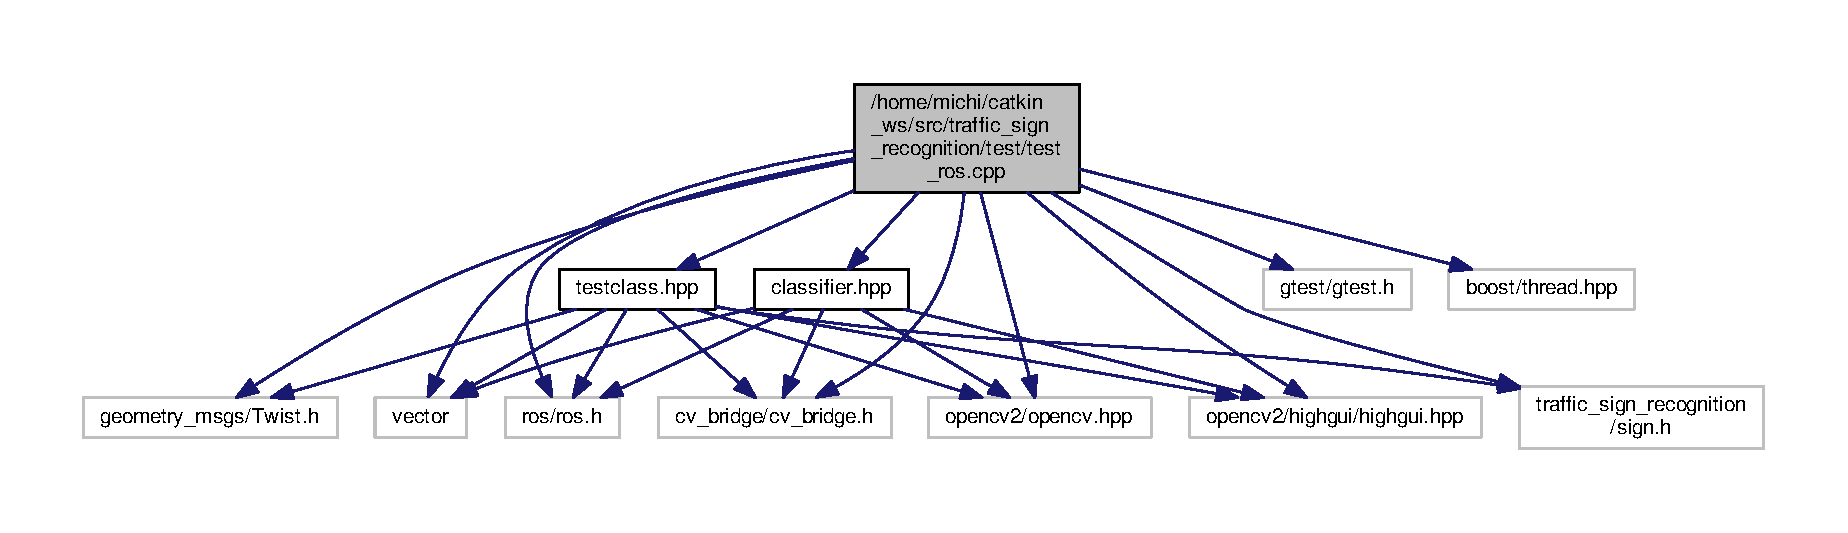
\includegraphics[width=350pt]{test__ros_8cpp__incl}
\end{center}
\end{figure}
\subsection*{Functions}
\begin{DoxyCompactItemize}
\item 
\hyperlink{test__ros_8cpp_ad7d6f768cb8051127ad20f4373997a58}{T\+E\+ST} (Test\+Ros, Pub\+Sub\+Test)
\begin{DoxyCompactList}\small\item\em Test subscriber and publisher to custom message sign. \end{DoxyCompactList}\item 
\hyperlink{test__ros_8cpp_a2034c9c2732910604b9e8ed8b995e1fc}{T\+E\+ST} (Test\+Ros, vel\+Test)
\begin{DoxyCompactList}\small\item\em Test velocity publisher. \end{DoxyCompactList}\item 
void \hyperlink{test__ros_8cpp_a46ca89271dcdb41dc6eea33f0e7ec218}{pthread} (void)
\begin{DoxyCompactList}\small\item\em Function that spins callbacks in tests. \end{DoxyCompactList}\item 
int \hyperlink{test__ros_8cpp_a3c04138a5bfe5d72780bb7e82a18e627}{main} (int argc, char $\ast$$\ast$argv)
\begin{DoxyCompactList}\small\item\em Main function that runs all tests in the file. \end{DoxyCompactList}\end{DoxyCompactItemize}


\subsection{Detailed Description}
Unit tests for publishers and subscribers. 

M\+IT License Copyright (c) 2017 Miguel Maestre Trueba Permission is hereby granted, free of charge, to any person obtaining a copy of this software and associated documentation files (the \char`\"{}\+Software\char`\"{}), to deal in the Software without restriction, including without limitation the rights to use, copy, modify, merge, publish, distribute, sublicense, and/or sell copies of the Software, and to permit persons to whom the Software is furnished to do so, subject to the following conditions\+: The above copyright notice and this permission notice shall be included in all copies or substantial portions of the Software. T\+HE S\+O\+F\+T\+W\+A\+RE IS P\+R\+O\+V\+I\+D\+ED \char`\"{}\+A\+S I\+S\char`\"{}, W\+I\+T\+H\+O\+UT W\+A\+R\+R\+A\+N\+TY OF A\+NY K\+I\+ND, E\+X\+P\+R\+E\+SS OR I\+M\+P\+L\+I\+ED, I\+N\+C\+L\+U\+D\+I\+NG B\+UT N\+OT L\+I\+M\+I\+T\+ED TO T\+HE W\+A\+R\+R\+A\+N\+T\+I\+ES OF M\+E\+R\+C\+H\+A\+N\+T\+A\+B\+I\+L\+I\+TY, F\+I\+T\+N\+E\+SS F\+OR A P\+A\+R\+T\+I\+C\+U\+L\+AR P\+U\+R\+P\+O\+SE A\+ND N\+O\+N\+I\+N\+F\+R\+I\+N\+G\+E\+M\+E\+NT. IN NO E\+V\+E\+NT S\+H\+A\+LL T\+HE A\+U\+T\+H\+O\+RS OR C\+O\+P\+Y\+R\+I\+G\+HT H\+O\+L\+D\+E\+RS BE L\+I\+A\+B\+LE F\+OR A\+NY C\+L\+A\+IM, D\+A\+M\+A\+G\+ES OR O\+T\+H\+ER L\+I\+A\+B\+I\+L\+I\+TY, W\+H\+E\+T\+H\+ER IN AN A\+C\+T\+I\+ON OF C\+O\+N\+T\+R\+A\+CT, T\+O\+RT OR O\+T\+H\+E\+R\+W\+I\+SE, A\+R\+I\+S\+I\+NG F\+R\+OM, O\+UT OF OR IN C\+O\+N\+N\+E\+C\+T\+I\+ON W\+I\+TH T\+HE S\+O\+F\+T\+W\+A\+RE OR T\+HE U\+SE OR O\+T\+H\+ER D\+E\+A\+L\+I\+N\+GS IN T\+HE S\+O\+F\+T\+W\+A\+RE.

\begin{DoxyCopyright}{Copyright}
Copyright 2017 Miguel Maestre Trueba
\end{DoxyCopyright}
\begin{DoxyAuthor}{Author}
Miguel Maestre Trueba 
\end{DoxyAuthor}


\subsection{Function Documentation}
\index{test\+\_\+ros.\+cpp@{test\+\_\+ros.\+cpp}!main@{main}}
\index{main@{main}!test\+\_\+ros.\+cpp@{test\+\_\+ros.\+cpp}}
\subsubsection[{\texorpdfstring{main(int argc, char $\ast$$\ast$argv)}{main(int argc, char **argv)}}]{\setlength{\rightskip}{0pt plus 5cm}int main (
\begin{DoxyParamCaption}
\item[{int}]{argc, }
\item[{char $\ast$$\ast$}]{argv}
\end{DoxyParamCaption}
)}\hypertarget{test__ros_8cpp_a3c04138a5bfe5d72780bb7e82a18e627}{}\label{test__ros_8cpp_a3c04138a5bfe5d72780bb7e82a18e627}


Main function that runs all tests in the file. 


\begin{DoxyParams}{Parameters}
{\em argc} & is the number of arguments \\
\hline
{\em argv} & is the arguments characters array \\
\hline
\end{DoxyParams}
\begin{DoxyReturn}{Returns}
Tests results 
\end{DoxyReturn}
\index{test\+\_\+ros.\+cpp@{test\+\_\+ros.\+cpp}!pthread@{pthread}}
\index{pthread@{pthread}!test\+\_\+ros.\+cpp@{test\+\_\+ros.\+cpp}}
\subsubsection[{\texorpdfstring{pthread(void)}{pthread(void)}}]{\setlength{\rightskip}{0pt plus 5cm}void pthread (
\begin{DoxyParamCaption}
\item[{void}]{}
\end{DoxyParamCaption}
)}\hypertarget{test__ros_8cpp_a46ca89271dcdb41dc6eea33f0e7ec218}{}\label{test__ros_8cpp_a46ca89271dcdb41dc6eea33f0e7ec218}


Function that spins callbacks in tests. 


\begin{DoxyParams}{Parameters}
{\em none} & \\
\hline
\end{DoxyParams}
\begin{DoxyReturn}{Returns}
none 
\end{DoxyReturn}
\index{test\+\_\+ros.\+cpp@{test\+\_\+ros.\+cpp}!T\+E\+ST@{T\+E\+ST}}
\index{T\+E\+ST@{T\+E\+ST}!test\+\_\+ros.\+cpp@{test\+\_\+ros.\+cpp}}
\subsubsection[{\texorpdfstring{T\+E\+S\+T(\+Test\+Ros, Pub\+Sub\+Test)}{TEST(TestRos, PubSubTest)}}]{\setlength{\rightskip}{0pt plus 5cm}T\+E\+ST (
\begin{DoxyParamCaption}
\item[{Test\+Ros}]{, }
\item[{Pub\+Sub\+Test}]{}
\end{DoxyParamCaption}
)}\hypertarget{test__ros_8cpp_ad7d6f768cb8051127ad20f4373997a58}{}\label{test__ros_8cpp_ad7d6f768cb8051127ad20f4373997a58}


Test subscriber and publisher to custom message sign. 


\begin{DoxyParams}{Parameters}
{\em none} & \\
\hline
\end{DoxyParams}
\begin{DoxyReturn}{Returns}
none 
\end{DoxyReturn}
\index{test\+\_\+ros.\+cpp@{test\+\_\+ros.\+cpp}!T\+E\+ST@{T\+E\+ST}}
\index{T\+E\+ST@{T\+E\+ST}!test\+\_\+ros.\+cpp@{test\+\_\+ros.\+cpp}}
\subsubsection[{\texorpdfstring{T\+E\+S\+T(\+Test\+Ros, vel\+Test)}{TEST(TestRos, velTest)}}]{\setlength{\rightskip}{0pt plus 5cm}T\+E\+ST (
\begin{DoxyParamCaption}
\item[{Test\+Ros}]{, }
\item[{vel\+Test}]{}
\end{DoxyParamCaption}
)}\hypertarget{test__ros_8cpp_a2034c9c2732910604b9e8ed8b995e1fc}{}\label{test__ros_8cpp_a2034c9c2732910604b9e8ed8b995e1fc}


Test velocity publisher. 


\begin{DoxyParams}{Parameters}
{\em none} & \\
\hline
\end{DoxyParams}
\begin{DoxyReturn}{Returns}
none 
\end{DoxyReturn}

\hypertarget{test__vision_8cpp}{}\section{/home/michi/catkin\+\_\+ws/src/traffic\+\_\+sign\+\_\+recognition/test/test\+\_\+vision.cpp File Reference}
\label{test__vision_8cpp}\index{/home/michi/catkin\+\_\+ws/src/traffic\+\_\+sign\+\_\+recognition/test/test\+\_\+vision.\+cpp@{/home/michi/catkin\+\_\+ws/src/traffic\+\_\+sign\+\_\+recognition/test/test\+\_\+vision.\+cpp}}


Unit test code for classifier class.  


{\ttfamily \#include $<$cv\+\_\+bridge/cv\+\_\+bridge.\+h$>$}\\*
{\ttfamily \#include $<$gtest/gtest.\+h$>$}\\*
{\ttfamily \#include $<$vector$>$}\\*
{\ttfamily \#include $<$opencv2/highgui/highgui.\+hpp$>$}\\*
{\ttfamily \#include \char`\"{}ros/ros.\+h\char`\"{}}\\*
{\ttfamily \#include \char`\"{}opencv2/opencv.\+hpp\char`\"{}}\\*
{\ttfamily \#include \char`\"{}classifier.\+hpp\char`\"{}}\\*
{\ttfamily \#include \char`\"{}traffic\+\_\+sign\+\_\+recognition/sign.\+h\char`\"{}}\\*
Include dependency graph for test\+\_\+vision.\+cpp\+:
\nopagebreak
\begin{figure}[H]
\begin{center}
\leavevmode
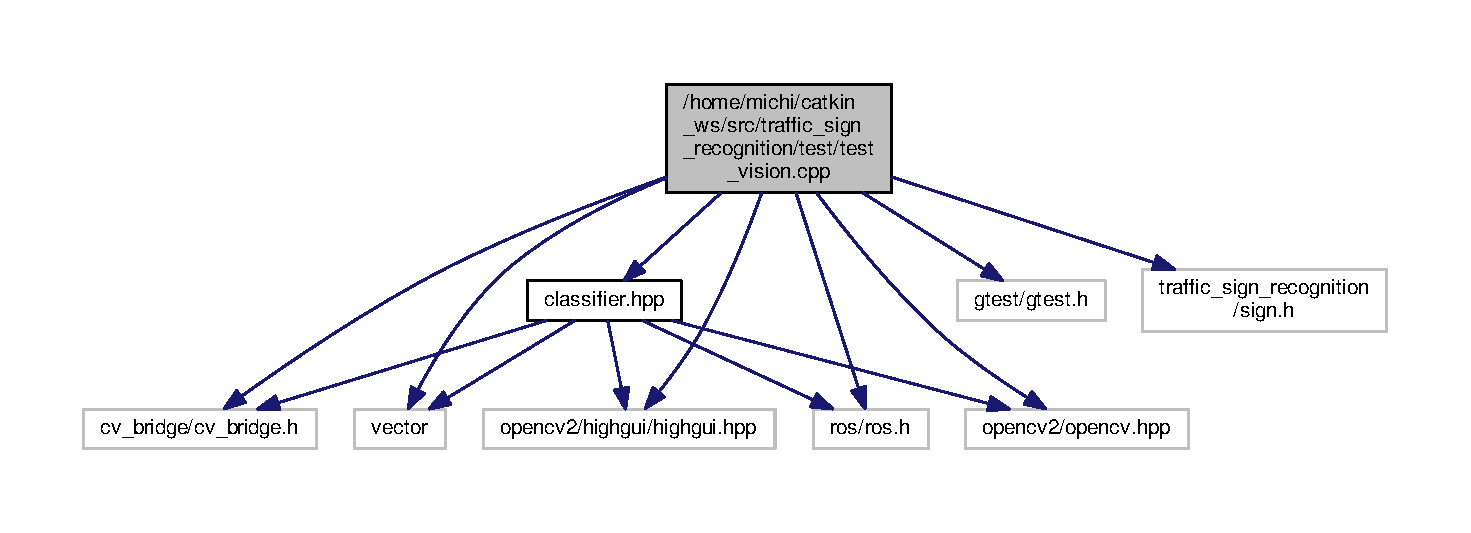
\includegraphics[width=350pt]{test__vision_8cpp__incl}
\end{center}
\end{figure}
\subsection*{Functions}
\begin{DoxyCompactItemize}
\item 
float \hyperlink{test__vision_8cpp_ad5fe7940ccf5aa5d83f0e38a9ee3956f}{testing\+\_\+stop} ()
\begin{DoxyCompactList}\small\item\em Function to test if stop sign is classified correctly. \end{DoxyCompactList}\item 
float \hyperlink{test__vision_8cpp_a584d210f5cc5c4276b76be620771776f}{testing\+\_\+turn} ()
\begin{DoxyCompactList}\small\item\em Function to test if turn sign is classified correctly. \end{DoxyCompactList}\item 
float \hyperlink{test__vision_8cpp_a25842fa907ae6cb50d47f14875747fd8}{testing\+\_\+forward} ()
\begin{DoxyCompactList}\small\item\em Function to test if forward sign is classified correctly. \end{DoxyCompactList}\item 
int \hyperlink{test__vision_8cpp_aa1b4dd9720020d5b21edfe84a44f01bc}{test\+\_\+training} ()
\begin{DoxyCompactList}\small\item\em Function to test if the S\+VM is trained correctly. \end{DoxyCompactList}\item 
std\+::vector$<$ cv\+::\+Mat $>$ \hyperlink{test__vision_8cpp_a3aba0acc0c91370fa0f55fde7d275d07}{test\+\_\+\+M\+S\+E\+R\+Good} ()
\begin{DoxyCompactList}\small\item\em Function to test if M\+S\+ER features are detected correctly in an image. \end{DoxyCompactList}\item 
std\+::vector$<$ cv\+::\+Mat $>$ \hyperlink{test__vision_8cpp_af43537cc188a5b7fe3b0f7816a2a3770}{test\+\_\+\+M\+S\+E\+R\+Bad} ()
\begin{DoxyCompactList}\small\item\em Function to test if M\+S\+ER features are not detected when not needed. \end{DoxyCompactList}\item 
cv\+::\+Mat \hyperlink{test__vision_8cpp_aa785afe838d8572d94763518f69f81dc}{test\+\_\+\+H\+OG} ()
\begin{DoxyCompactList}\small\item\em Function to test if H\+OG features detected correctly. \end{DoxyCompactList}\item 
int \hyperlink{test__vision_8cpp_aaefc04db3ab6b68dd277ed31617ea312}{test\+\_\+viz} (int type)
\begin{DoxyCompactList}\small\item\em Function to test visualization conditions work. \end{DoxyCompactList}\item 
\hyperlink{test__vision_8cpp_ad4a11d70b4b64471d459267f05f28683}{T\+E\+ST} (Test\+Vision, stop\+Test)
\begin{DoxyCompactList}\small\item\em Test if stop sign is being classified correctly. \end{DoxyCompactList}\item 
\hyperlink{test__vision_8cpp_a9831814400e08bfec821e8792fb029df}{T\+E\+ST} (Test\+Vision, turn\+Test)
\begin{DoxyCompactList}\small\item\em Test if turn sign is being classified correctly. \end{DoxyCompactList}\item 
\hyperlink{test__vision_8cpp_a4ff7ce997129f9fb6f4e2c7a1960b657}{T\+E\+ST} (Test\+Vision, forward\+Test)
\begin{DoxyCompactList}\small\item\em Test if forward sign is being classified correctly. \end{DoxyCompactList}\item 
\hyperlink{test__vision_8cpp_a0134157d34a5ae4e8a11860926e88613}{T\+E\+ST} (Test\+Vision, training\+Test)
\begin{DoxyCompactList}\small\item\em Test if S\+VM training correctly. \end{DoxyCompactList}\item 
\hyperlink{test__vision_8cpp_aa77ceaaf170bd3e57228630ce8ff24cb}{T\+E\+ST} (Test\+Vision, M\+S\+E\+R\+Tests)
\begin{DoxyCompactList}\small\item\em Tests to see if M\+S\+ER features are being detected and not detected properly. \end{DoxyCompactList}\item 
\hyperlink{test__vision_8cpp_ab3b529599b7622ac876ea2beba5f56fa}{T\+E\+ST} (Test\+Vision, H\+O\+G\+Test)
\begin{DoxyCompactList}\small\item\em Test to see that H\+OG features are being processed properly. \end{DoxyCompactList}\item 
\hyperlink{test__vision_8cpp_a223cb3c9f50bc327f39d663a3fb2e94c}{T\+E\+ST} (Test\+Vision, Viz\+Test)
\begin{DoxyCompactList}\small\item\em Test to check if visualization is acting correctly. \end{DoxyCompactList}\item 
int \hyperlink{test__vision_8cpp_a3c04138a5bfe5d72780bb7e82a18e627}{main} (int argc, char $\ast$$\ast$argv)
\begin{DoxyCompactList}\small\item\em Main function that runs all tests in the file. \end{DoxyCompactList}\end{DoxyCompactItemize}


\subsection{Detailed Description}
Unit test code for classifier class. 

M\+IT License Copyright (c) 2017 Miguel Maestre Trueba Permission is hereby granted, free of charge, to any person obtaining a copy of this software and associated documentation files (the \char`\"{}\+Software\char`\"{}), to deal in the Software without restriction, including without limitation the rights to use, copy, modify, merge, publish, distribute, sublicense, and/or sell copies of the Software, and to permit persons to whom the Software is furnished to do so, subject to the following conditions\+: The above copyright notice and this permission notice shall be included in all copies or substantial portions of the Software. T\+HE S\+O\+F\+T\+W\+A\+RE IS P\+R\+O\+V\+I\+D\+ED \char`\"{}\+A\+S I\+S\char`\"{}, W\+I\+T\+H\+O\+UT W\+A\+R\+R\+A\+N\+TY OF A\+NY K\+I\+ND, E\+X\+P\+R\+E\+SS OR I\+M\+P\+L\+I\+ED, I\+N\+C\+L\+U\+D\+I\+NG B\+UT N\+OT L\+I\+M\+I\+T\+ED TO T\+HE W\+A\+R\+R\+A\+N\+T\+I\+ES OF M\+E\+R\+C\+H\+A\+N\+T\+A\+B\+I\+L\+I\+TY, F\+I\+T\+N\+E\+SS F\+OR A P\+A\+R\+T\+I\+C\+U\+L\+AR P\+U\+R\+P\+O\+SE A\+ND N\+O\+N\+I\+N\+F\+R\+I\+N\+G\+E\+M\+E\+NT. IN NO E\+V\+E\+NT S\+H\+A\+LL T\+HE A\+U\+T\+H\+O\+RS OR C\+O\+P\+Y\+R\+I\+G\+HT H\+O\+L\+D\+E\+RS BE L\+I\+A\+B\+LE F\+OR A\+NY C\+L\+A\+IM, D\+A\+M\+A\+G\+ES OR O\+T\+H\+ER L\+I\+A\+B\+I\+L\+I\+TY, W\+H\+E\+T\+H\+ER IN AN A\+C\+T\+I\+ON OF C\+O\+N\+T\+R\+A\+CT, T\+O\+RT OR O\+T\+H\+E\+R\+W\+I\+SE, A\+R\+I\+S\+I\+NG F\+R\+OM, O\+UT OF OR IN C\+O\+N\+N\+E\+C\+T\+I\+ON W\+I\+TH T\+HE S\+O\+F\+T\+W\+A\+RE OR T\+HE U\+SE OR O\+T\+H\+ER D\+E\+A\+L\+I\+N\+GS IN T\+HE S\+O\+F\+T\+W\+A\+RE.

\begin{DoxyCopyright}{Copyright}
Copyright 2017 Miguel Maestre Trueba
\end{DoxyCopyright}
\begin{DoxyAuthor}{Author}
Miguel Maestre Trueba 
\end{DoxyAuthor}


\subsection{Function Documentation}
\index{test\+\_\+vision.\+cpp@{test\+\_\+vision.\+cpp}!main@{main}}
\index{main@{main}!test\+\_\+vision.\+cpp@{test\+\_\+vision.\+cpp}}
\subsubsection[{\texorpdfstring{main(int argc, char $\ast$$\ast$argv)}{main(int argc, char **argv)}}]{\setlength{\rightskip}{0pt plus 5cm}int main (
\begin{DoxyParamCaption}
\item[{int}]{argc, }
\item[{char $\ast$$\ast$}]{argv}
\end{DoxyParamCaption}
)}\hypertarget{test__vision_8cpp_a3c04138a5bfe5d72780bb7e82a18e627}{}\label{test__vision_8cpp_a3c04138a5bfe5d72780bb7e82a18e627}


Main function that runs all tests in the file. 


\begin{DoxyParams}{Parameters}
{\em argc} & is the number of arguments \\
\hline
{\em argv} & is the arguments characters array \\
\hline
\end{DoxyParams}
\begin{DoxyReturn}{Returns}
Tests results 
\end{DoxyReturn}
\index{test\+\_\+vision.\+cpp@{test\+\_\+vision.\+cpp}!T\+E\+ST@{T\+E\+ST}}
\index{T\+E\+ST@{T\+E\+ST}!test\+\_\+vision.\+cpp@{test\+\_\+vision.\+cpp}}
\subsubsection[{\texorpdfstring{T\+E\+S\+T(\+Test\+Vision, stop\+Test)}{TEST(TestVision, stopTest)}}]{\setlength{\rightskip}{0pt plus 5cm}T\+E\+ST (
\begin{DoxyParamCaption}
\item[{Test\+Vision}]{, }
\item[{stop\+Test}]{}
\end{DoxyParamCaption}
)}\hypertarget{test__vision_8cpp_ad4a11d70b4b64471d459267f05f28683}{}\label{test__vision_8cpp_ad4a11d70b4b64471d459267f05f28683}


Test if stop sign is being classified correctly. 


\begin{DoxyParams}{Parameters}
{\em none} & \\
\hline
\end{DoxyParams}
\begin{DoxyReturn}{Returns}
none 
\end{DoxyReturn}
\index{test\+\_\+vision.\+cpp@{test\+\_\+vision.\+cpp}!T\+E\+ST@{T\+E\+ST}}
\index{T\+E\+ST@{T\+E\+ST}!test\+\_\+vision.\+cpp@{test\+\_\+vision.\+cpp}}
\subsubsection[{\texorpdfstring{T\+E\+S\+T(\+Test\+Vision, turn\+Test)}{TEST(TestVision, turnTest)}}]{\setlength{\rightskip}{0pt plus 5cm}T\+E\+ST (
\begin{DoxyParamCaption}
\item[{Test\+Vision}]{, }
\item[{turn\+Test}]{}
\end{DoxyParamCaption}
)}\hypertarget{test__vision_8cpp_a9831814400e08bfec821e8792fb029df}{}\label{test__vision_8cpp_a9831814400e08bfec821e8792fb029df}


Test if turn sign is being classified correctly. 


\begin{DoxyParams}{Parameters}
{\em none} & \\
\hline
\end{DoxyParams}
\begin{DoxyReturn}{Returns}
none 
\end{DoxyReturn}
\index{test\+\_\+vision.\+cpp@{test\+\_\+vision.\+cpp}!T\+E\+ST@{T\+E\+ST}}
\index{T\+E\+ST@{T\+E\+ST}!test\+\_\+vision.\+cpp@{test\+\_\+vision.\+cpp}}
\subsubsection[{\texorpdfstring{T\+E\+S\+T(\+Test\+Vision, forward\+Test)}{TEST(TestVision, forwardTest)}}]{\setlength{\rightskip}{0pt plus 5cm}T\+E\+ST (
\begin{DoxyParamCaption}
\item[{Test\+Vision}]{, }
\item[{forward\+Test}]{}
\end{DoxyParamCaption}
)}\hypertarget{test__vision_8cpp_a4ff7ce997129f9fb6f4e2c7a1960b657}{}\label{test__vision_8cpp_a4ff7ce997129f9fb6f4e2c7a1960b657}


Test if forward sign is being classified correctly. 


\begin{DoxyParams}{Parameters}
{\em none} & \\
\hline
\end{DoxyParams}
\begin{DoxyReturn}{Returns}
none 
\end{DoxyReturn}
\index{test\+\_\+vision.\+cpp@{test\+\_\+vision.\+cpp}!T\+E\+ST@{T\+E\+ST}}
\index{T\+E\+ST@{T\+E\+ST}!test\+\_\+vision.\+cpp@{test\+\_\+vision.\+cpp}}
\subsubsection[{\texorpdfstring{T\+E\+S\+T(\+Test\+Vision, training\+Test)}{TEST(TestVision, trainingTest)}}]{\setlength{\rightskip}{0pt plus 5cm}T\+E\+ST (
\begin{DoxyParamCaption}
\item[{Test\+Vision}]{, }
\item[{training\+Test}]{}
\end{DoxyParamCaption}
)}\hypertarget{test__vision_8cpp_a0134157d34a5ae4e8a11860926e88613}{}\label{test__vision_8cpp_a0134157d34a5ae4e8a11860926e88613}


Test if S\+VM training correctly. 


\begin{DoxyParams}{Parameters}
{\em none} & \\
\hline
\end{DoxyParams}
\begin{DoxyReturn}{Returns}
none 
\end{DoxyReturn}
\index{test\+\_\+vision.\+cpp@{test\+\_\+vision.\+cpp}!T\+E\+ST@{T\+E\+ST}}
\index{T\+E\+ST@{T\+E\+ST}!test\+\_\+vision.\+cpp@{test\+\_\+vision.\+cpp}}
\subsubsection[{\texorpdfstring{T\+E\+S\+T(\+Test\+Vision, M\+S\+E\+R\+Tests)}{TEST(TestVision, MSERTests)}}]{\setlength{\rightskip}{0pt plus 5cm}T\+E\+ST (
\begin{DoxyParamCaption}
\item[{Test\+Vision}]{, }
\item[{M\+S\+E\+R\+Tests}]{}
\end{DoxyParamCaption}
)}\hypertarget{test__vision_8cpp_aa77ceaaf170bd3e57228630ce8ff24cb}{}\label{test__vision_8cpp_aa77ceaaf170bd3e57228630ce8ff24cb}


Tests to see if M\+S\+ER features are being detected and not detected properly. 


\begin{DoxyParams}{Parameters}
{\em none} & \\
\hline
\end{DoxyParams}
\begin{DoxyReturn}{Returns}
none 
\end{DoxyReturn}
\index{test\+\_\+vision.\+cpp@{test\+\_\+vision.\+cpp}!T\+E\+ST@{T\+E\+ST}}
\index{T\+E\+ST@{T\+E\+ST}!test\+\_\+vision.\+cpp@{test\+\_\+vision.\+cpp}}
\subsubsection[{\texorpdfstring{T\+E\+S\+T(\+Test\+Vision, H\+O\+G\+Test)}{TEST(TestVision, HOGTest)}}]{\setlength{\rightskip}{0pt plus 5cm}T\+E\+ST (
\begin{DoxyParamCaption}
\item[{Test\+Vision}]{, }
\item[{H\+O\+G\+Test}]{}
\end{DoxyParamCaption}
)}\hypertarget{test__vision_8cpp_ab3b529599b7622ac876ea2beba5f56fa}{}\label{test__vision_8cpp_ab3b529599b7622ac876ea2beba5f56fa}


Test to see that H\+OG features are being processed properly. 


\begin{DoxyParams}{Parameters}
{\em none} & \\
\hline
\end{DoxyParams}
\begin{DoxyReturn}{Returns}
none 
\end{DoxyReturn}
\index{test\+\_\+vision.\+cpp@{test\+\_\+vision.\+cpp}!T\+E\+ST@{T\+E\+ST}}
\index{T\+E\+ST@{T\+E\+ST}!test\+\_\+vision.\+cpp@{test\+\_\+vision.\+cpp}}
\subsubsection[{\texorpdfstring{T\+E\+S\+T(\+Test\+Vision, Viz\+Test)}{TEST(TestVision, VizTest)}}]{\setlength{\rightskip}{0pt plus 5cm}T\+E\+ST (
\begin{DoxyParamCaption}
\item[{Test\+Vision}]{, }
\item[{Viz\+Test}]{}
\end{DoxyParamCaption}
)}\hypertarget{test__vision_8cpp_a223cb3c9f50bc327f39d663a3fb2e94c}{}\label{test__vision_8cpp_a223cb3c9f50bc327f39d663a3fb2e94c}


Test to check if visualization is acting correctly. 


\begin{DoxyParams}{Parameters}
{\em none} & \\
\hline
\end{DoxyParams}
\begin{DoxyReturn}{Returns}
none 
\end{DoxyReturn}
\index{test\+\_\+vision.\+cpp@{test\+\_\+vision.\+cpp}!test\+\_\+\+H\+OG@{test\+\_\+\+H\+OG}}
\index{test\+\_\+\+H\+OG@{test\+\_\+\+H\+OG}!test\+\_\+vision.\+cpp@{test\+\_\+vision.\+cpp}}
\subsubsection[{\texorpdfstring{test\+\_\+\+H\+O\+G()}{test_HOG()}}]{\setlength{\rightskip}{0pt plus 5cm}cv\+::\+Mat test\+\_\+\+H\+OG (
\begin{DoxyParamCaption}
{}
\end{DoxyParamCaption}
)}\hypertarget{test__vision_8cpp_aa785afe838d8572d94763518f69f81dc}{}\label{test__vision_8cpp_aa785afe838d8572d94763518f69f81dc}


Function to test if H\+OG features detected correctly. 


\begin{DoxyParams}{Parameters}
{\em none} & \\
\hline
\end{DoxyParams}
\begin{DoxyReturn}{Returns}
Matrix of 81x1 with the H\+OG descriptor 
\end{DoxyReturn}
\index{test\+\_\+vision.\+cpp@{test\+\_\+vision.\+cpp}!test\+\_\+\+M\+S\+E\+R\+Bad@{test\+\_\+\+M\+S\+E\+R\+Bad}}
\index{test\+\_\+\+M\+S\+E\+R\+Bad@{test\+\_\+\+M\+S\+E\+R\+Bad}!test\+\_\+vision.\+cpp@{test\+\_\+vision.\+cpp}}
\subsubsection[{\texorpdfstring{test\+\_\+\+M\+S\+E\+R\+Bad()}{test_MSERBad()}}]{\setlength{\rightskip}{0pt plus 5cm}std\+::vector$<$cv\+::\+Mat$>$ test\+\_\+\+M\+S\+E\+R\+Bad (
\begin{DoxyParamCaption}
{}
\end{DoxyParamCaption}
)}\hypertarget{test__vision_8cpp_af43537cc188a5b7fe3b0f7816a2a3770}{}\label{test__vision_8cpp_af43537cc188a5b7fe3b0f7816a2a3770}


Function to test if M\+S\+ER features are not detected when not needed. 


\begin{DoxyParams}{Parameters}
{\em none} & \\
\hline
\end{DoxyParams}
\begin{DoxyReturn}{Returns}
Empty vector of images 
\end{DoxyReturn}
\index{test\+\_\+vision.\+cpp@{test\+\_\+vision.\+cpp}!test\+\_\+\+M\+S\+E\+R\+Good@{test\+\_\+\+M\+S\+E\+R\+Good}}
\index{test\+\_\+\+M\+S\+E\+R\+Good@{test\+\_\+\+M\+S\+E\+R\+Good}!test\+\_\+vision.\+cpp@{test\+\_\+vision.\+cpp}}
\subsubsection[{\texorpdfstring{test\+\_\+\+M\+S\+E\+R\+Good()}{test_MSERGood()}}]{\setlength{\rightskip}{0pt plus 5cm}std\+::vector$<$cv\+::\+Mat$>$ test\+\_\+\+M\+S\+E\+R\+Good (
\begin{DoxyParamCaption}
{}
\end{DoxyParamCaption}
)}\hypertarget{test__vision_8cpp_a3aba0acc0c91370fa0f55fde7d275d07}{}\label{test__vision_8cpp_a3aba0acc0c91370fa0f55fde7d275d07}


Function to test if M\+S\+ER features are detected correctly in an image. 


\begin{DoxyParams}{Parameters}
{\em none} & \\
\hline
\end{DoxyParams}
\begin{DoxyReturn}{Returns}
Set of images with the detections 
\end{DoxyReturn}
\index{test\+\_\+vision.\+cpp@{test\+\_\+vision.\+cpp}!test\+\_\+training@{test\+\_\+training}}
\index{test\+\_\+training@{test\+\_\+training}!test\+\_\+vision.\+cpp@{test\+\_\+vision.\+cpp}}
\subsubsection[{\texorpdfstring{test\+\_\+training()}{test_training()}}]{\setlength{\rightskip}{0pt plus 5cm}int test\+\_\+training (
\begin{DoxyParamCaption}
{}
\end{DoxyParamCaption}
)}\hypertarget{test__vision_8cpp_aa1b4dd9720020d5b21edfe84a44f01bc}{}\label{test__vision_8cpp_aa1b4dd9720020d5b21edfe84a44f01bc}


Function to test if the S\+VM is trained correctly. 


\begin{DoxyParams}{Parameters}
{\em none} & \\
\hline
\end{DoxyParams}
\begin{DoxyReturn}{Returns}
1 if succeeds 
\end{DoxyReturn}
\index{test\+\_\+vision.\+cpp@{test\+\_\+vision.\+cpp}!test\+\_\+viz@{test\+\_\+viz}}
\index{test\+\_\+viz@{test\+\_\+viz}!test\+\_\+vision.\+cpp@{test\+\_\+vision.\+cpp}}
\subsubsection[{\texorpdfstring{test\+\_\+viz(int type)}{test_viz(int type)}}]{\setlength{\rightskip}{0pt plus 5cm}int test\+\_\+viz (
\begin{DoxyParamCaption}
\item[{int}]{type}
\end{DoxyParamCaption}
)}\hypertarget{test__vision_8cpp_aaefc04db3ab6b68dd277ed31617ea312}{}\label{test__vision_8cpp_aaefc04db3ab6b68dd277ed31617ea312}


Function to test visualization conditions work. 


\begin{DoxyParams}{Parameters}
{\em type} & is the type of sign detected \\
\hline
\end{DoxyParams}
\begin{DoxyReturn}{Returns}
int indicating type of sign plotted 
\end{DoxyReturn}
\index{test\+\_\+vision.\+cpp@{test\+\_\+vision.\+cpp}!testing\+\_\+forward@{testing\+\_\+forward}}
\index{testing\+\_\+forward@{testing\+\_\+forward}!test\+\_\+vision.\+cpp@{test\+\_\+vision.\+cpp}}
\subsubsection[{\texorpdfstring{testing\+\_\+forward()}{testing_forward()}}]{\setlength{\rightskip}{0pt plus 5cm}float testing\+\_\+forward (
\begin{DoxyParamCaption}
{}
\end{DoxyParamCaption}
)}\hypertarget{test__vision_8cpp_a25842fa907ae6cb50d47f14875747fd8}{}\label{test__vision_8cpp_a25842fa907ae6cb50d47f14875747fd8}


Function to test if forward sign is classified correctly. 


\begin{DoxyParams}{Parameters}
{\em none} & \\
\hline
\end{DoxyParams}
\begin{DoxyReturn}{Returns}
Label of the classified sign 
\end{DoxyReturn}
\index{test\+\_\+vision.\+cpp@{test\+\_\+vision.\+cpp}!testing\+\_\+stop@{testing\+\_\+stop}}
\index{testing\+\_\+stop@{testing\+\_\+stop}!test\+\_\+vision.\+cpp@{test\+\_\+vision.\+cpp}}
\subsubsection[{\texorpdfstring{testing\+\_\+stop()}{testing_stop()}}]{\setlength{\rightskip}{0pt plus 5cm}float testing\+\_\+stop (
\begin{DoxyParamCaption}
{}
\end{DoxyParamCaption}
)}\hypertarget{test__vision_8cpp_ad5fe7940ccf5aa5d83f0e38a9ee3956f}{}\label{test__vision_8cpp_ad5fe7940ccf5aa5d83f0e38a9ee3956f}


Function to test if stop sign is classified correctly. 


\begin{DoxyParams}{Parameters}
{\em none} & \\
\hline
\end{DoxyParams}
\begin{DoxyReturn}{Returns}
Label of the classified sign 
\end{DoxyReturn}
\index{test\+\_\+vision.\+cpp@{test\+\_\+vision.\+cpp}!testing\+\_\+turn@{testing\+\_\+turn}}
\index{testing\+\_\+turn@{testing\+\_\+turn}!test\+\_\+vision.\+cpp@{test\+\_\+vision.\+cpp}}
\subsubsection[{\texorpdfstring{testing\+\_\+turn()}{testing_turn()}}]{\setlength{\rightskip}{0pt plus 5cm}float testing\+\_\+turn (
\begin{DoxyParamCaption}
{}
\end{DoxyParamCaption}
)}\hypertarget{test__vision_8cpp_a584d210f5cc5c4276b76be620771776f}{}\label{test__vision_8cpp_a584d210f5cc5c4276b76be620771776f}


Function to test if turn sign is classified correctly. 


\begin{DoxyParams}{Parameters}
{\em none} & \\
\hline
\end{DoxyParams}
\begin{DoxyReturn}{Returns}
Label of the classified sign 
\end{DoxyReturn}

\hypertarget{testclass_8cpp}{}\section{/home/michi/catkin\+\_\+ws/src/traffic\+\_\+sign\+\_\+recognition/test/testclass.cpp File Reference}
\label{testclass_8cpp}\index{/home/michi/catkin\+\_\+ws/src/traffic\+\_\+sign\+\_\+recognition/test/testclass.\+cpp@{/home/michi/catkin\+\_\+ws/src/traffic\+\_\+sign\+\_\+recognition/test/testclass.\+cpp}}


Implementation of the methods of class testclass.  


{\ttfamily \#include $<$cv\+\_\+bridge/cv\+\_\+bridge.\+h$>$}\\*
{\ttfamily \#include $<$geometry\+\_\+msgs/\+Twist.\+h$>$}\\*
{\ttfamily \#include $<$cstdlib$>$}\\*
{\ttfamily \#include $<$string$>$}\\*
{\ttfamily \#include $<$opencv2/highgui/highgui.\+hpp$>$}\\*
{\ttfamily \#include \char`\"{}ros/ros.\+h\char`\"{}}\\*
{\ttfamily \#include \char`\"{}opencv2/opencv.\+hpp\char`\"{}}\\*
{\ttfamily \#include \char`\"{}ros/console.\+h\char`\"{}}\\*
{\ttfamily \#include \char`\"{}traffic\+\_\+sign\+\_\+recognition/sign.\+h\char`\"{}}\\*
{\ttfamily \#include \char`\"{}testclass.\+hpp\char`\"{}}\\*
Include dependency graph for testclass.\+cpp\+:
\nopagebreak
\begin{figure}[H]
\begin{center}
\leavevmode
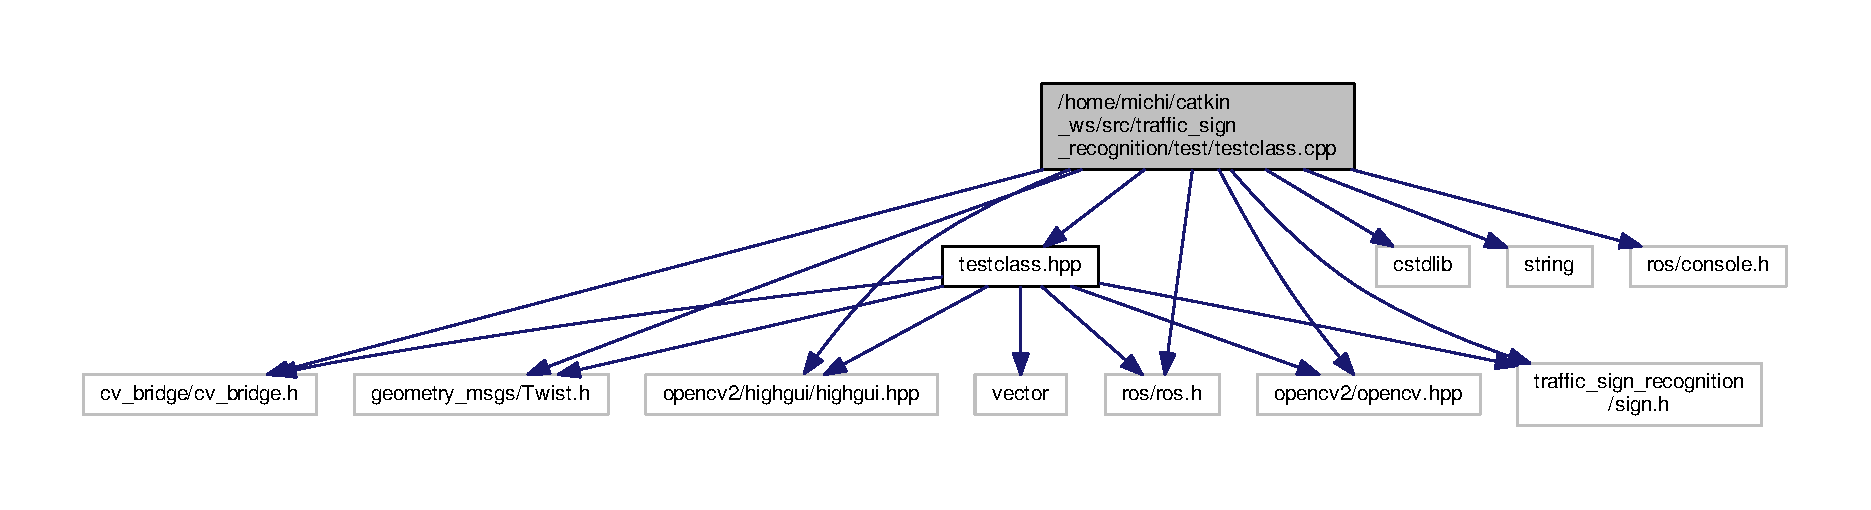
\includegraphics[width=350pt]{testclass_8cpp__incl}
\end{center}
\end{figure}


\subsection{Detailed Description}
Implementation of the methods of class testclass. 

M\+IT License Copyright (c) 2017 Miguel Maestre Trueba Permission is hereby granted, free of charge, to any person obtaining a copy of this software and associated documentation files (the \char`\"{}\+Software\char`\"{}), to deal in the Software without restriction, including without limitation the rights to use, copy, modify, merge, publish, distribute, sublicense, and/or sell copies of the Software, and to permit persons to whom the Software is furnished to do so, subject to the following conditions\+: The above copyright notice and this permission notice shall be included in all copies or substantial portions of the Software. T\+HE S\+O\+F\+T\+W\+A\+RE IS P\+R\+O\+V\+I\+D\+ED \char`\"{}\+A\+S I\+S\char`\"{}, W\+I\+T\+H\+O\+UT W\+A\+R\+R\+A\+N\+TY OF A\+NY K\+I\+ND, E\+X\+P\+R\+E\+SS OR I\+M\+P\+L\+I\+ED, I\+N\+C\+L\+U\+D\+I\+NG B\+UT N\+OT L\+I\+M\+I\+T\+ED TO T\+HE W\+A\+R\+R\+A\+N\+T\+I\+ES OF M\+E\+R\+C\+H\+A\+N\+T\+A\+B\+I\+L\+I\+TY, F\+I\+T\+N\+E\+SS F\+OR A P\+A\+R\+T\+I\+C\+U\+L\+AR P\+U\+R\+P\+O\+SE A\+ND N\+O\+N\+I\+N\+F\+R\+I\+N\+G\+E\+M\+E\+NT. IN NO E\+V\+E\+NT S\+H\+A\+LL T\+HE A\+U\+T\+H\+O\+RS OR C\+O\+P\+Y\+R\+I\+G\+HT H\+O\+L\+D\+E\+RS BE L\+I\+A\+B\+LE F\+OR A\+NY C\+L\+A\+IM, D\+A\+M\+A\+G\+ES OR O\+T\+H\+ER L\+I\+A\+B\+I\+L\+I\+TY, W\+H\+E\+T\+H\+ER IN AN A\+C\+T\+I\+ON OF C\+O\+N\+T\+R\+A\+CT, T\+O\+RT OR O\+T\+H\+E\+R\+W\+I\+SE, A\+R\+I\+S\+I\+NG F\+R\+OM, O\+UT OF OR IN C\+O\+N\+N\+E\+C\+T\+I\+ON W\+I\+TH T\+HE S\+O\+F\+T\+W\+A\+RE OR T\+HE U\+SE OR O\+T\+H\+ER D\+E\+A\+L\+I\+N\+GS IN T\+HE S\+O\+F\+T\+W\+A\+RE.

\begin{DoxyCopyright}{Copyright}
Copyright 2017 Miguel Maestre Trueba
\end{DoxyCopyright}
\begin{DoxyAuthor}{Author}
Miguel Maestre Trueba 
\end{DoxyAuthor}

\hypertarget{testclass_8hpp}{}\section{/home/michi/catkin\+\_\+ws/src/traffic\+\_\+sign\+\_\+recognition/test/testclass.hpp File Reference}
\label{testclass_8hpp}\index{/home/michi/catkin\+\_\+ws/src/traffic\+\_\+sign\+\_\+recognition/test/testclass.\+hpp@{/home/michi/catkin\+\_\+ws/src/traffic\+\_\+sign\+\_\+recognition/test/testclass.\+hpp}}


Definition for class testclass.  


{\ttfamily \#include $<$cv\+\_\+bridge/cv\+\_\+bridge.\+h$>$}\\*
{\ttfamily \#include $<$geometry\+\_\+msgs/\+Twist.\+h$>$}\\*
{\ttfamily \#include $<$vector$>$}\\*
{\ttfamily \#include $<$opencv2/highgui/highgui.\+hpp$>$}\\*
{\ttfamily \#include \char`\"{}opencv2/opencv.\+hpp\char`\"{}}\\*
{\ttfamily \#include \char`\"{}ros/ros.\+h\char`\"{}}\\*
{\ttfamily \#include \char`\"{}traffic\+\_\+sign\+\_\+recognition/sign.\+h\char`\"{}}\\*
Include dependency graph for testclass.\+hpp\+:
\nopagebreak
\begin{figure}[H]
\begin{center}
\leavevmode
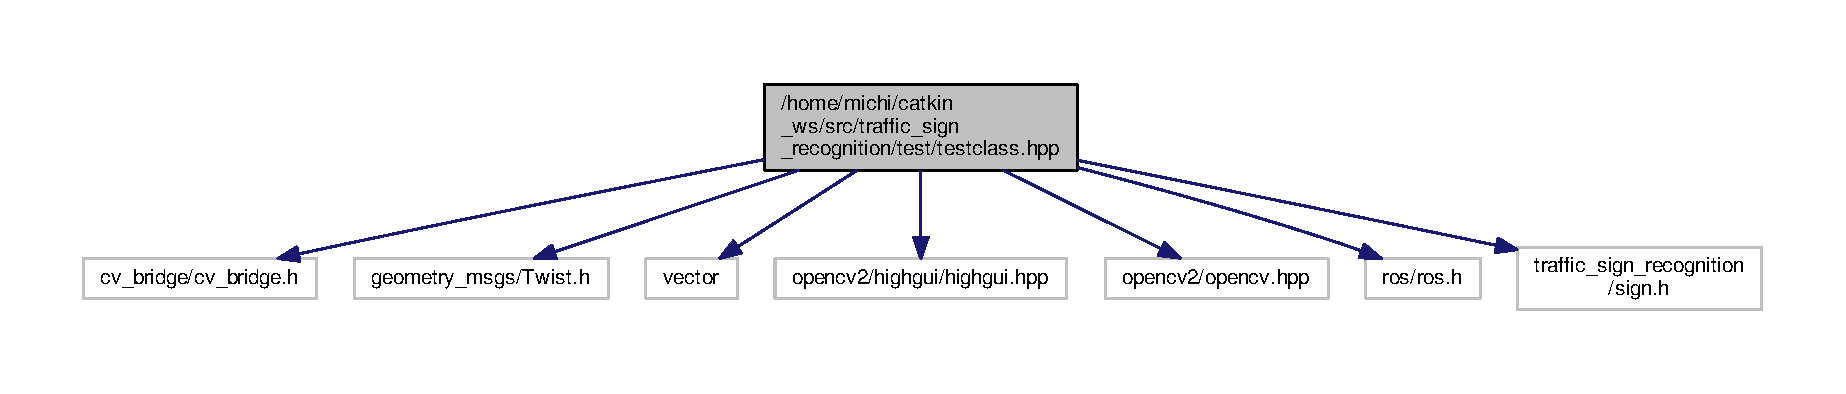
\includegraphics[width=350pt]{testclass_8hpp__incl}
\end{center}
\end{figure}
This graph shows which files directly or indirectly include this file\+:
\nopagebreak
\begin{figure}[H]
\begin{center}
\leavevmode
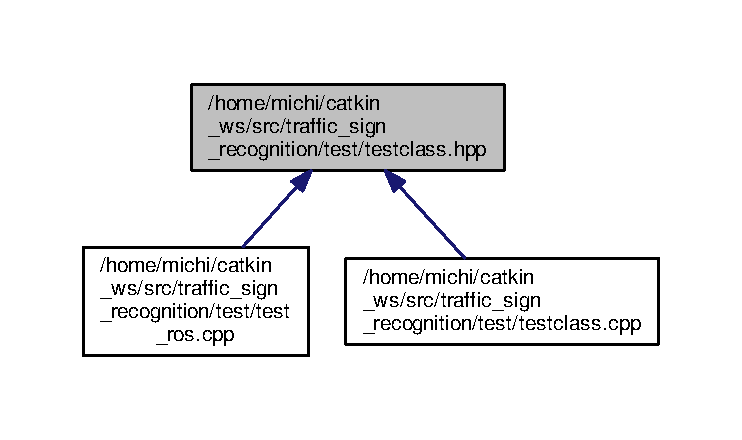
\includegraphics[width=350pt]{testclass_8hpp__dep__incl}
\end{center}
\end{figure}
\subsection*{Classes}
\begin{DoxyCompactItemize}
\item 
class \hyperlink{classtestclass}{testclass}
\begin{DoxyCompactList}\small\item\em Definition of the testclass class. It contains mock callbacks to test publishers and subscribers. \end{DoxyCompactList}\end{DoxyCompactItemize}


\subsection{Detailed Description}
Definition for class testclass. 

M\+IT License Copyright (c) 2017 Miguel Maestre Trueba Permission is hereby granted, free of charge, to any person obtaining a copy of this software and associated documentation files (the \char`\"{}\+Software\char`\"{}), to deal in the Software without restriction, including without limitation the rights to use, copy, modify, merge, publish, distribute, sublicense, and/or sell copies of the Software, and to permit persons to whom the Software is furnished to do so, subject to the following conditions\+: The above copyright notice and this permission notice shall be included in all copies or substantial portions of the Software. T\+HE S\+O\+F\+T\+W\+A\+RE IS P\+R\+O\+V\+I\+D\+ED \char`\"{}\+A\+S I\+S\char`\"{}, W\+I\+T\+H\+O\+UT W\+A\+R\+R\+A\+N\+TY OF A\+NY K\+I\+ND, E\+X\+P\+R\+E\+SS OR I\+M\+P\+L\+I\+ED, I\+N\+C\+L\+U\+D\+I\+NG B\+UT N\+OT L\+I\+M\+I\+T\+ED TO T\+HE W\+A\+R\+R\+A\+N\+T\+I\+ES OF M\+E\+R\+C\+H\+A\+N\+T\+A\+B\+I\+L\+I\+TY, F\+I\+T\+N\+E\+SS F\+OR A P\+A\+R\+T\+I\+C\+U\+L\+AR P\+U\+R\+P\+O\+SE A\+ND N\+O\+N\+I\+N\+F\+R\+I\+N\+G\+E\+M\+E\+NT. IN NO E\+V\+E\+NT S\+H\+A\+LL T\+HE A\+U\+T\+H\+O\+RS OR C\+O\+P\+Y\+R\+I\+G\+HT H\+O\+L\+D\+E\+RS BE L\+I\+A\+B\+LE F\+OR A\+NY C\+L\+A\+IM, D\+A\+M\+A\+G\+ES OR O\+T\+H\+ER L\+I\+A\+B\+I\+L\+I\+TY, W\+H\+E\+T\+H\+ER IN AN A\+C\+T\+I\+ON OF C\+O\+N\+T\+R\+A\+CT, T\+O\+RT OR O\+T\+H\+E\+R\+W\+I\+SE, A\+R\+I\+S\+I\+NG F\+R\+OM, O\+UT OF OR IN C\+O\+N\+N\+E\+C\+T\+I\+ON W\+I\+TH T\+HE S\+O\+F\+T\+W\+A\+RE OR T\+HE U\+SE OR O\+T\+H\+ER D\+E\+A\+L\+I\+N\+GS IN T\+HE S\+O\+F\+T\+W\+A\+RE.

\begin{DoxyCopyright}{Copyright}
Copyright 2017 Miguel Maestre Trueba
\end{DoxyCopyright}
\begin{DoxyAuthor}{Author}
Miguel Maestre Trueba 
\end{DoxyAuthor}

%--- End generated contents ---

% Index
\backmatter
\newpage
\phantomsection
\clearemptydoublepage
\addcontentsline{toc}{chapter}{Index}
\printindex

\end{document}
